\documentclass[]{book}
\usepackage{lmodern}
\usepackage{amssymb,amsmath}
\usepackage{ifxetex,ifluatex}
\usepackage{fixltx2e} % provides \textsubscript
\ifnum 0\ifxetex 1\fi\ifluatex 1\fi=0 % if pdftex
  \usepackage[T1]{fontenc}
  \usepackage[utf8]{inputenc}
\else % if luatex or xelatex
  \ifxetex
    \usepackage{mathspec}
  \else
    \usepackage{fontspec}
  \fi
  \defaultfontfeatures{Ligatures=TeX,Scale=MatchLowercase}
\fi
% use upquote if available, for straight quotes in verbatim environments
\IfFileExists{upquote.sty}{\usepackage{upquote}}{}
% use microtype if available
\IfFileExists{microtype.sty}{%
\usepackage{microtype}
\UseMicrotypeSet[protrusion]{basicmath} % disable protrusion for tt fonts
}{}
\usepackage[margin=1in]{geometry}
\usepackage{hyperref}
\hypersetup{unicode=true,
            pdftitle={A brief introduction to QGIS},
            pdfauthor={Ivan Viveros Santos},
            pdfborder={0 0 0},
            breaklinks=true}
\urlstyle{same}  % don't use monospace font for urls
\usepackage{natbib}
\bibliographystyle{apalike}
\usepackage{longtable,booktabs}
\usepackage{graphicx,grffile}
\makeatletter
\def\maxwidth{\ifdim\Gin@nat@width>\linewidth\linewidth\else\Gin@nat@width\fi}
\def\maxheight{\ifdim\Gin@nat@height>\textheight\textheight\else\Gin@nat@height\fi}
\makeatother
% Scale images if necessary, so that they will not overflow the page
% margins by default, and it is still possible to overwrite the defaults
% using explicit options in \includegraphics[width, height, ...]{}
\setkeys{Gin}{width=\maxwidth,height=\maxheight,keepaspectratio}
\IfFileExists{parskip.sty}{%
\usepackage{parskip}
}{% else
\setlength{\parindent}{0pt}
\setlength{\parskip}{6pt plus 2pt minus 1pt}
}
\setlength{\emergencystretch}{3em}  % prevent overfull lines
\providecommand{\tightlist}{%
  \setlength{\itemsep}{0pt}\setlength{\parskip}{0pt}}
\setcounter{secnumdepth}{5}
% Redefines (sub)paragraphs to behave more like sections
\ifx\paragraph\undefined\else
\let\oldparagraph\paragraph
\renewcommand{\paragraph}[1]{\oldparagraph{#1}\mbox{}}
\fi
\ifx\subparagraph\undefined\else
\let\oldsubparagraph\subparagraph
\renewcommand{\subparagraph}[1]{\oldsubparagraph{#1}\mbox{}}
\fi

%%% Use protect on footnotes to avoid problems with footnotes in titles
\let\rmarkdownfootnote\footnote%
\def\footnote{\protect\rmarkdownfootnote}

%%% Change title format to be more compact
\usepackage{titling}

% Create subtitle command for use in maketitle
\newcommand{\subtitle}[1]{
  \posttitle{
    \begin{center}\large#1\end{center}
    }
}

\setlength{\droptitle}{-2em}

  \title{A brief introduction to QGIS}
    \pretitle{\vspace{\droptitle}\centering\huge}
  \posttitle{\par}
    \author{Ivan Viveros Santos}
    \preauthor{\centering\large\emph}
  \postauthor{\par}
      \predate{\centering\large\emph}
  \postdate{\par}
    \date{2019-09-23}

\usepackage{booktabs}
\usepackage{amsthm}
\makeatletter
\def\thm@space@setup{%
  \thm@preskip=8pt plus 2pt minus 4pt
  \thm@postskip=\thm@preskip
}
\makeatother

\usepackage{amsthm}
\newtheorem{theorem}{Theorem}[chapter]
\newtheorem{lemma}{Lemma}[chapter]
\theoremstyle{definition}
\newtheorem{definition}{Definition}[chapter]
\newtheorem{corollary}{Corollary}[chapter]
\newtheorem{proposition}{Proposition}[chapter]
\theoremstyle{definition}
\newtheorem{example}{Example}[chapter]
\theoremstyle{definition}
\newtheorem{exercise}{Exercise}[chapter]
\theoremstyle{remark}
\newtheorem*{remark}{Remark}
\newtheorem*{solution}{Solution}
\begin{document}
\maketitle

{
\setcounter{tocdepth}{1}
\tableofcontents
}
\chapter{Introduction}\label{introduction}

\href{https://qgis.org/en/site/}{QGIS} is an Open Source Geographic
Information System (GIS) licensed under the GNU General Public License.

The aim of this document is to present some recipes about importing and
exporting vectors, and treatment and exploration of spatial data. I plan
to add more recipes on vector styling and map composition.

This is a brief introduction to QGIS, as such, it does not replace in
any maner the \href{https://docs.qgis.org/3.4/en/docs/user_manual/}{QGIS
User Guide}. I also recommend you visiting the
\href{https://gis.stackexchange.com/}{StackExchange} chanel, where you
can get support on questions related to QGIS.

The data used to illustrate the recipes presented in this document come
from the \href{http://donnees.ville.montreal.qc.ca/}{Portail données
ouvertes Montréal}; particularly, the selected data from this site is
under the license
\href{https://creativecommons.org/licenses/by/4.0/}{Creative Commons
Attribution 4.0 International}.

To follow the recipes presented in this document, please download the
accompanying files from my
\href{https://github.com/iviveros/QGIS_Data}{GitHub page}.

\chapter{QGIS installation and Graphical User
Interface}\label{installation}

\section{QGIS installation}\label{qgis-installation}

It is possible to install QGIS on Windows, Mac OS X, Linux, BSD, and
Android operating systems. The installers can be downloaded from
\href{https://qgis.org/en/site/forusers/download.html}{this website},
and \href{https://qgis.org/en/site/forusers/alldownloads.html\#}{this
link} provides detailed installation instructions.

By the time of writing this document, the last version of QGIS is
\texttt{3.8.2\ Zanzibar}, which was released on October 16, 2019.

\section{QGIS Graphical User
Interface}\label{qgis-graphical-user-interface}

The QGIS graphical user interface (GUI) is composed of:

\begin{itemize}
\tightlist
\item
  \textbf{Menu bar}: gives access to the main functionalities of QGIS.
\item
  \textbf{Toolbars}: give a quick access to QGIS functionalities.
\item
  \textbf{Panels}: they provide several functionalities, for instance
  managing layers, and browsing spatial data.
\item
  \textbf{Map display}: shows the spatial data of the current project.
\end{itemize}

\begin{figure}

{\centering 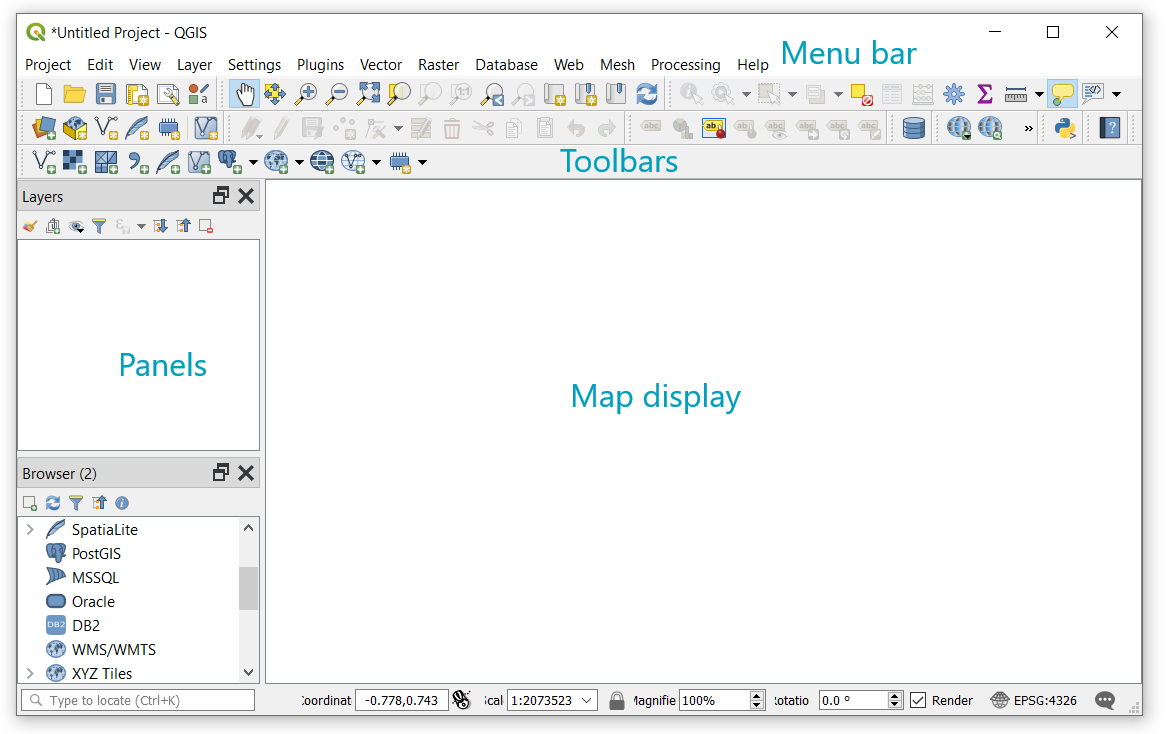
\includegraphics[width=16.19in]{figures/QGIS_interface} 

}

\caption{QGIS GUI}\label{fig:unnamed-chunk-1}
\end{figure}

It is possible to customize the appearance of QGIS by navigating to
\textbf{View} from the \textbf{Menu bar}. From here, you can select the
panels and toolbars you want to display. I would recommend toggling the
\textbf{Processing Toolbox} from the panel because it allows to quickly
access to the main operations available in QGIS.

\chapter{Loading and Exporting data}\label{loading-and-exporting-data}

The quickest way to load data into QGIS is the technique drag-and-drop.
It only requires locating the data you want to import into QGIS, select
the file, and drop it on the \textbf{Map display} or on the
\textbf{layer panel}.

Another option for importing data is to use the browser panel. Navigate
through the browser, locate the layer or data to be imported,
right-click on it, and finally select Add Layer to Project. However,
using the \textbf{Manage Layers Toolbar} or \textbf{Add Layer} from the
\textbf{Layer} menu give more control on the importation.

\section{Importing data from text
files}\label{importing-data-from-text-files}

This recipe is illustrated with the
\texttt{coordonnees-stations-rsqa.csv} file, which reports the locations
of the stations of the Air Quality Monitoring Network (RSQA) set up in
Montreal. The aim of the
\href{https://ville.montreal.qc.ca/rapportmontrealdurable/en/air-quality.php}{RSQA}
is to monitor the atmospheric concentration of
\href{https://www.epa.gov/criteria-air-pollutants}{criteria pollutants}.

\begin{enumerate}
\def\labelenumi{\arabic{enumi}.}
\tightlist
\item
  Navigate to the \textbf{Layer} menu and select \textbf{Add delimited
  text layer}. The following dialog will pop up:
\end{enumerate}

\begin{figure}

{\centering 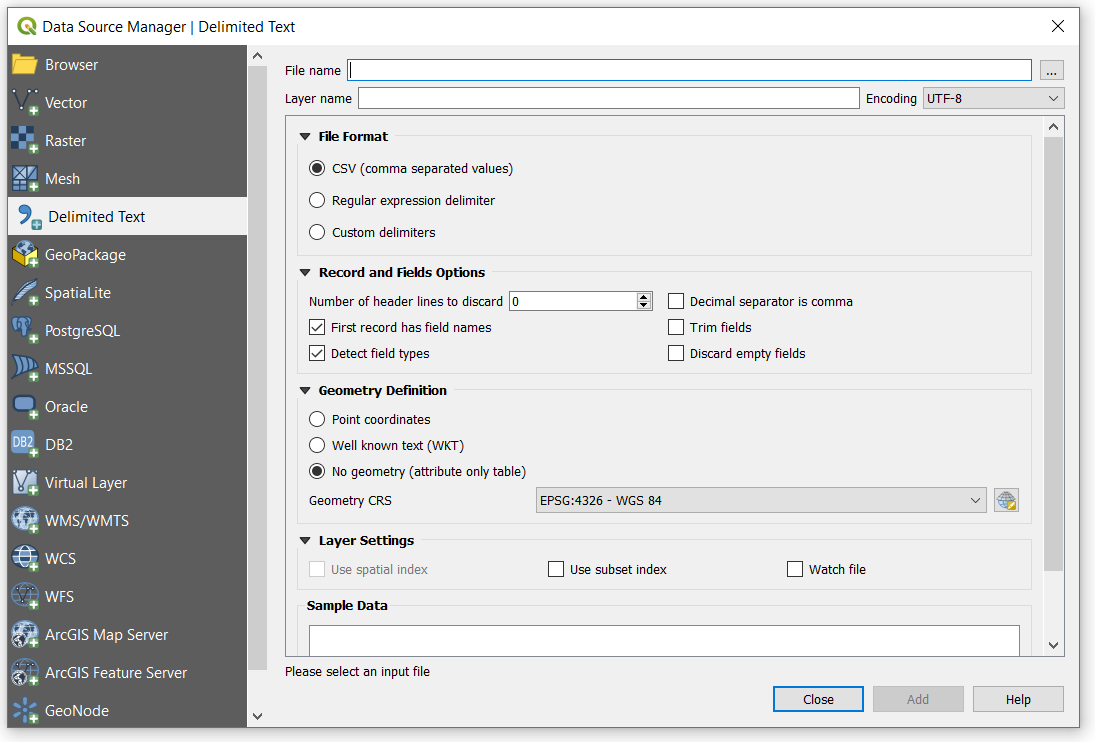
\includegraphics[width=15.21in]{figures/Delimited_Text_Dialog} 

}

\caption{Add delimited text layer window}\label{fig:unnamed-chunk-2}
\end{figure}

\begin{enumerate}
\def\labelenumi{\arabic{enumi}.}
\setcounter{enumi}{1}
\tightlist
\item
  In the \textbf{File Name} field, indicate the path to the
  \texttt{coordonnees-stations-rsqa.csv} file.
\end{enumerate}

\begin{figure}

{\centering 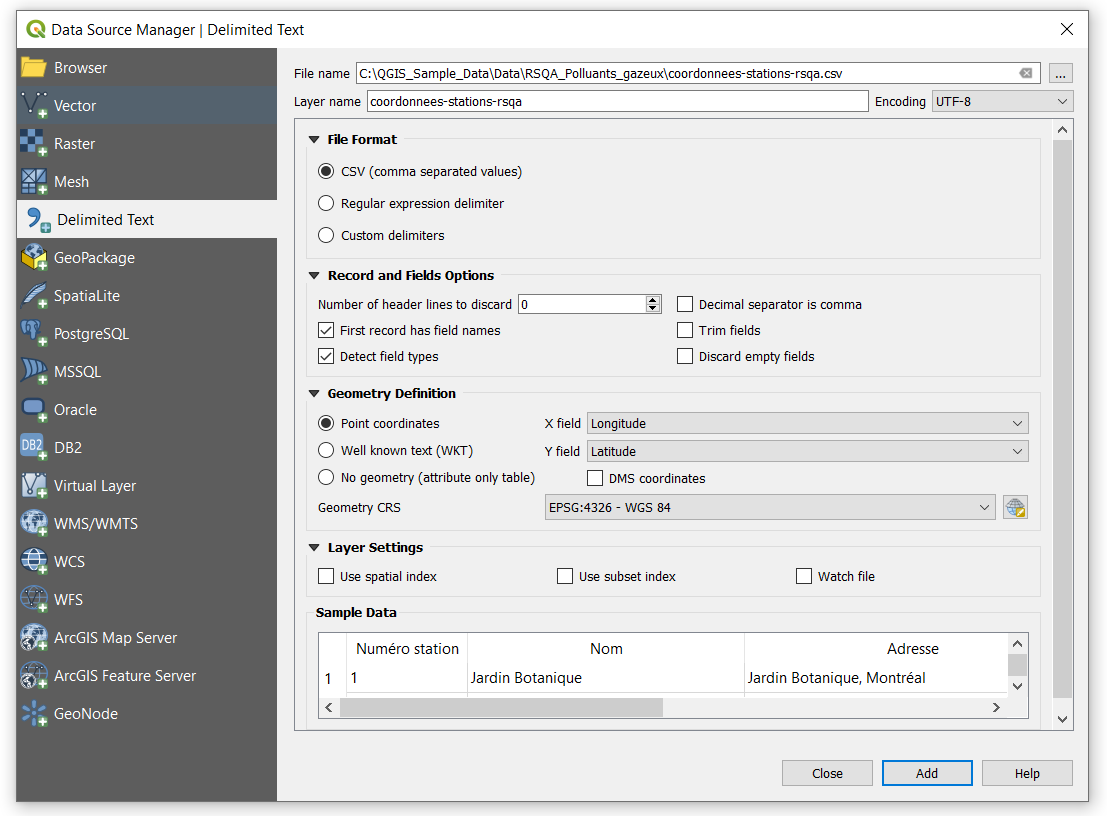
\includegraphics[width=15.38in]{figures/Delimited_Text_Dialog_2} 

}

\caption{Indicating the path to the text file}\label{fig:unnamed-chunk-3}
\end{figure}

\begin{enumerate}
\def\labelenumi{\arabic{enumi}.}
\setcounter{enumi}{2}
\item
  In the \textbf{Geometry Definition} section, indicate that point
  coordinates are being imported. Then indicate the corresponding fields
  for longitude and latitude. According to the sources of the layer
  being imported, the coordinate system is WGS 84, so we don't need to
  change it. When you want to import an attribute table, you can select
  the option \textbf{No geometry}.
\item
  Click on \textbf{Add}. You will see the following set of points,
  probably not in the same colour. Optionally, you can add a base map or
  another layer to give some spatial context, but for now we have
  successfully imported the layer corresponding to the stations of the
  RSQA network.
\end{enumerate}

\begin{figure}

{\centering 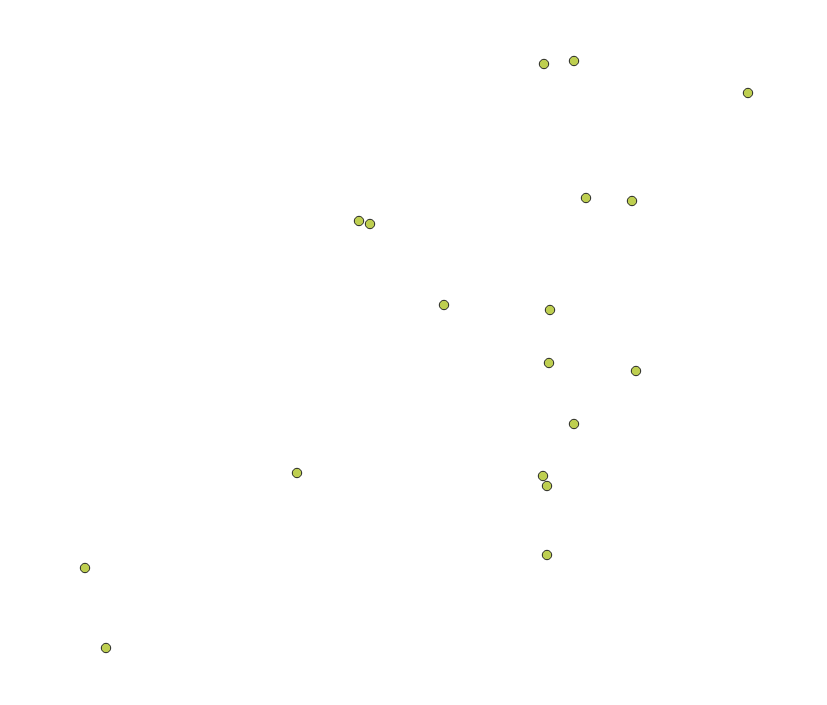
\includegraphics[width=11.49in]{figures/Stations_RSQA} 

}

\caption{Montreal's Air Quality Monitoring Network}\label{fig:unnamed-chunk-4}
\end{figure}

\begin{quote}
In section \ref{basemaps} we describe how to add a basemap to add
spatial context.
\end{quote}

\begin{enumerate}
\def\labelenumi{\arabic{enumi}.}
\setcounter{enumi}{4}
\tightlist
\item
  \textbf{Optional step}: save the imported layer as a new shapefile
  (Section \ref{saveLayer}).
\end{enumerate}

\section{Importing data from KML
files}\label{importing-data-from-kml-files}

QGIS supports importing
\href{https://developers.google.com/kml/}{Keyhole Markup Language} (KML)
files. KML is the format used by Google Earth to show spatial data.

The importation of a KML is illustrated with the \texttt{grandparcs.kml}
file which contains polygons corresponding to the
\href{http://donnees.ville.montreal.qc.ca/dataset/grands-parcs}{parks of
Montreal}.

\begin{enumerate}
\def\labelenumi{\arabic{enumi}.}
\tightlist
\item
  Navigate to the \textbf{Layer} menu and select \textbf{Add vector
  layer}. The following dialog will pop up:
\end{enumerate}

\begin{figure}

{\centering 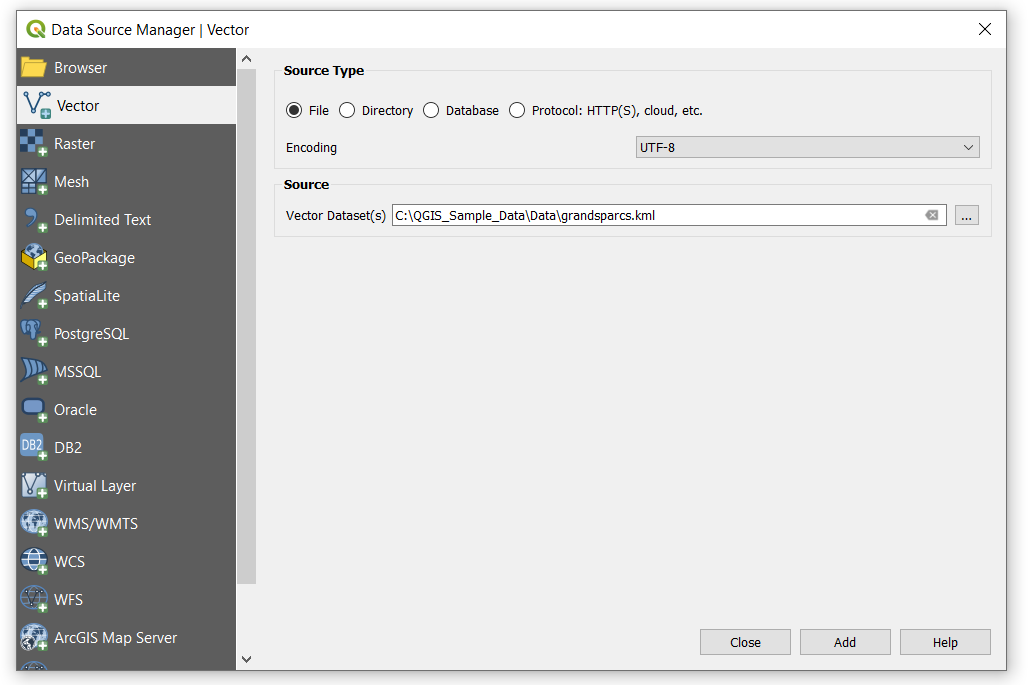
\includegraphics[width=14.32in]{figures/Import_KML} 

}

\caption{Add vector layer window}\label{fig:unnamed-chunk-5}
\end{figure}

\begin{enumerate}
\def\labelenumi{\arabic{enumi}.}
\setcounter{enumi}{1}
\tightlist
\item
  In the \textbf{File Name} field, indicate the path to the
  \texttt{grandparcs.kml} file. The following layer will be displayed in
  QGIS:
\end{enumerate}

\begin{figure}

{\centering 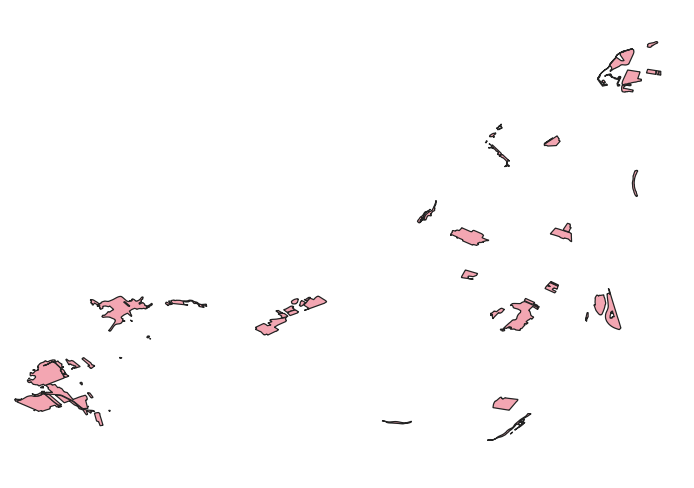
\includegraphics[width=9.64in]{figures/Import_KML_2} 

}

\caption{Montreal's parks}\label{fig:unnamed-chunk-6}
\end{figure}

\section{Importing GeoJSON files}\label{importing-geojson-files}

\href{https://geojson.org/}{GeoJSON} is another frequently used format
for storing and representing geographical attributes. This format is
based on the JavaScript Object Notation (JSON).

The importation of a GeoJSON layer is illustrated with the
\texttt{ilotschaleur.json} file. This file contains the
\href{http://donnees.ville.montreal.qc.ca/dataset/schema-environnement-milieux-naturels/resource/8cd8d34a-cfdd-4acf-a363-d4adaeff18c0}{urban
heat islands (UHI) of Montreal}. UHI correspond to urban areas
characterized by higher summer temperatures than the immediate
environment with differences between 5 and 10°C.

\begin{enumerate}
\def\labelenumi{\arabic{enumi}.}
\tightlist
\item
  Navigate to the \textbf{Layer} menu and select \textbf{Add vector
  layer}. The following dialog will pop up:
\end{enumerate}

\begin{figure}

{\centering 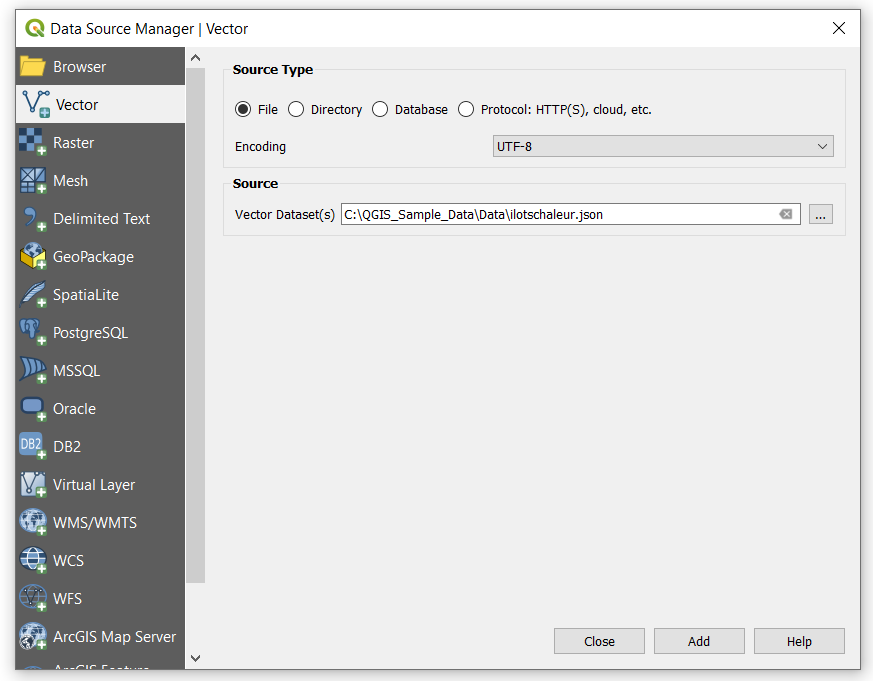
\includegraphics[width=12.12in]{figures/Import_geojson} 

}

\caption{Add vector layer window}\label{fig:unnamed-chunk-7}
\end{figure}

\begin{enumerate}
\def\labelenumi{\arabic{enumi}.}
\setcounter{enumi}{1}
\tightlist
\item
  In the \textbf{File Name} field, indicate the path to the
  \texttt{ilotschaleur.json} file. The following layer will be displayed
  in QGIS:
\end{enumerate}

\begin{figure}

{\centering 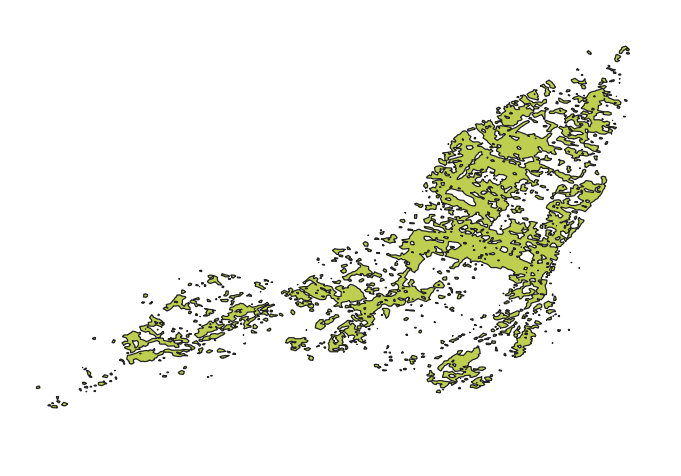
\includegraphics[width=9.46in]{figures/Import_geojson_2} 

}

\caption{Urban heat islands (UHI) of Montreal}\label{fig:unnamed-chunk-8}
\end{figure}

\section{Saving a layer}\label{saveLayer}

We use the previously imported \texttt{coordonnees-stations-rsqa.csv}
file to illustrate how to export a layer in a different format.

\begin{enumerate}
\def\labelenumi{\arabic{enumi}.}
\tightlist
\item
  Right-click on the name of the layer, select \textbf{Export}, then
  \textbf{Save features As\ldots{}} The following dialog window will pop
  up.
\end{enumerate}

\begin{figure}

{\centering 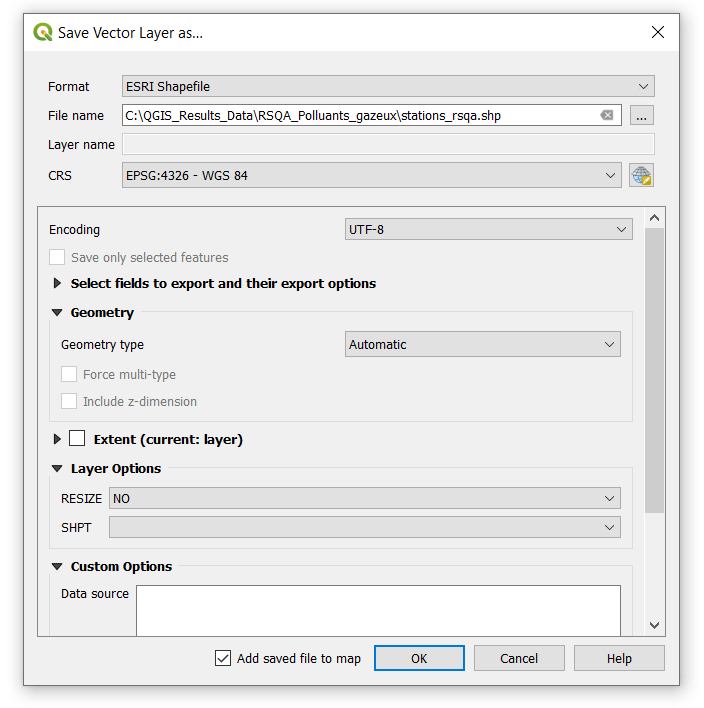
\includegraphics[width=9.78in]{figures/Save_Layer} 

}

\caption{Save features as... window}\label{fig:unnamed-chunk-9}
\end{figure}

\begin{enumerate}
\def\labelenumi{\arabic{enumi}.}
\setcounter{enumi}{1}
\item
  Select the format in which you want to export the layer. In this case,
  we have selected the widely used ESRI shapefile, we will use this
  layer in future recipes. Another commonly used format is GeoJson since
  it is compatible with web base applications.
\item
  Indicate the path where the layer will be stored and give it a name.
  Indicate whether you want to add the saved file to the current
  project, and finally click on OK.
\end{enumerate}

\section{Reprojecting a layer}\label{reprojecting-a-layer}

Most of the time, the layers are not in a CRS that is more convenient
for the operation in hand. QGIS offers on-the-fly reprojections for
rendering the layers. However, when executing operations like spatial
analysis, it is required that all layers be in the same CRS. This recipe
is illustrated with the \texttt{LIMADMIN.shp} file that corresponds to
the administrative limits of Montreal's boroughs.

Before executing a spatial analysis, it is recommended to reproject the
layers to the most convenient CRS.

\begin{enumerate}
\def\labelenumi{\arabic{enumi}.}
\tightlist
\item
  Right-click on the name of the layer, select \textbf{Export}, then
  \textbf{Save features As\ldots{}}. The following dialog window will
  pop up.
\item
  Indicate the path where the layer will be stored and give it a name.
  If you tick the box \textbf{Add saved file to map}, the recently
  exported layer will be saved and added to the current project.
\end{enumerate}

\begin{figure}

{\centering 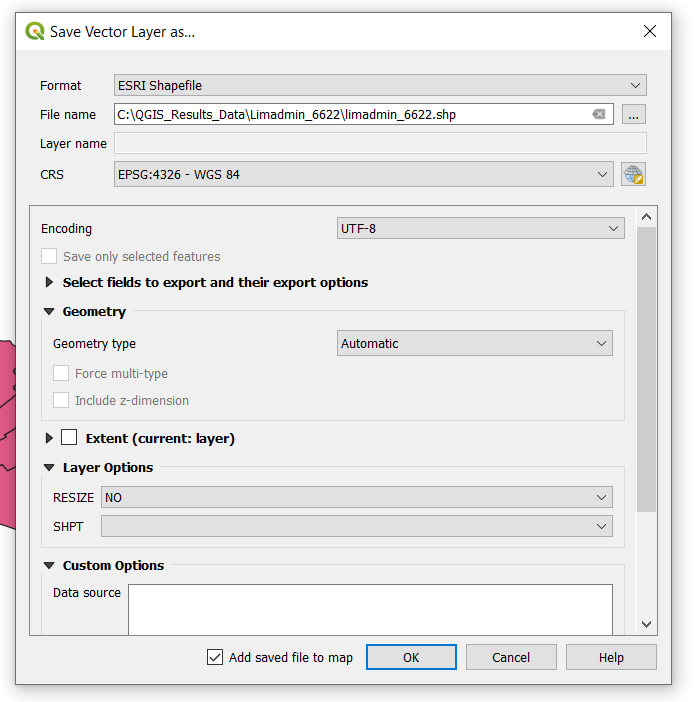
\includegraphics[width=9.64in]{figures/Reproject_Layer} 

}

\caption{Reprojecting a layer}\label{fig:unnamed-chunk-10}
\end{figure}

\begin{enumerate}
\def\labelenumi{\arabic{enumi}.}
\setcounter{enumi}{2}
\tightlist
\item
  Click on the little globe to select the CRS in which the new layer
  will be projected. The following window will pop up:
\end{enumerate}

\begin{figure}

{\centering 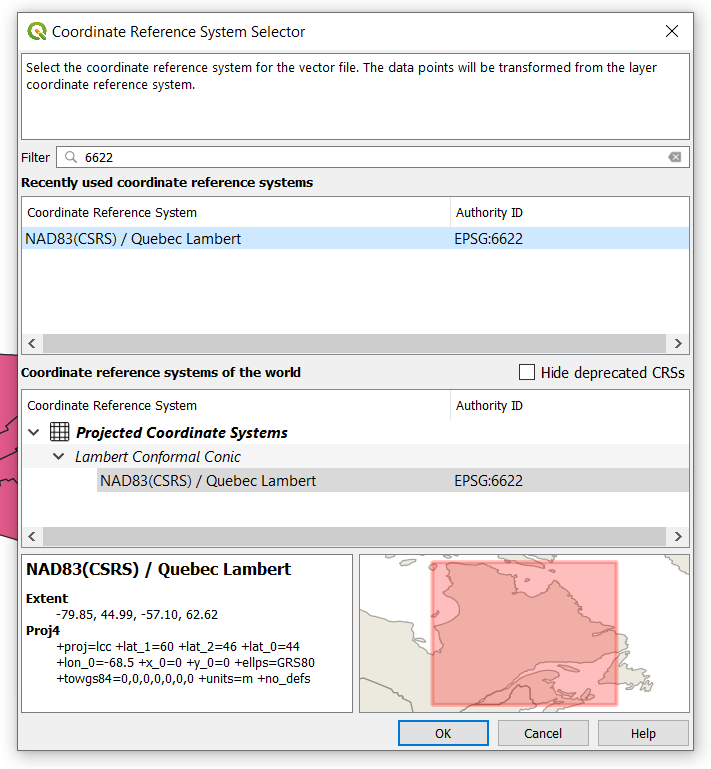
\includegraphics[width=9.88in]{figures/Reproject_Layer_CRS} 

}

\caption{Selecting another CRS}\label{fig:unnamed-chunk-11}
\end{figure}

\begin{enumerate}
\def\labelenumi{\arabic{enumi}.}
\setcounter{enumi}{3}
\tightlist
\item
  You can filter the CRS. In this case we will export the new layer in
  \textbf{EPSG:6622}, since it is the most accurate for
  \href{https://epsg.io/6622}{Quebec}. Click \textbf{OK} to confirm the
  selection of the CRS and click again \textbf{OK} to save the layer.
\end{enumerate}

\chapter{Data treatment}\label{data-treatment}

\section{Joining a layer data}\label{joining-a-layer-data}

Another frequent task before executing spatial analysis with QGIS is to
join an attribute table to a layer.

To illustrate this task, we refer to the \texttt{stations\_rsqa.shp}
file generated in section 1 and the file
\texttt{pollutants\_average\_12\_31\_2019\_13H.csv} file. When we load
the shapefile into QGIS we identify that this layer only contains
information on the identification and location of stations that compose
the Air Quality Monitoring Network (RSQA).

\begin{figure}

{\centering 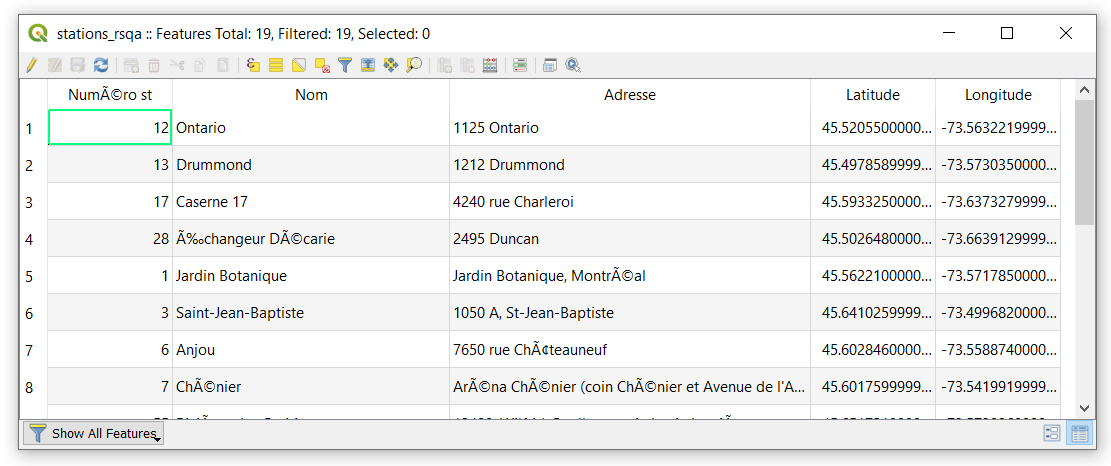
\includegraphics[width=15.43in]{figures/Change_Encoding} 

}

\caption{Attribute table of stations}\label{fig:unnamed-chunk-12}
\end{figure}

We realize another problem, the name (nom) and the address of the
stations are not correctly displayed. In order to fix it, right-click on
the name of the layer, and select properties. A window will pop up. Go
to \textbf{Source} and change the \textbf{Data Source Encoding} to
\textbf{UTF-8}. Finally, click on Apply to accept the changes.

\begin{figure}

{\centering 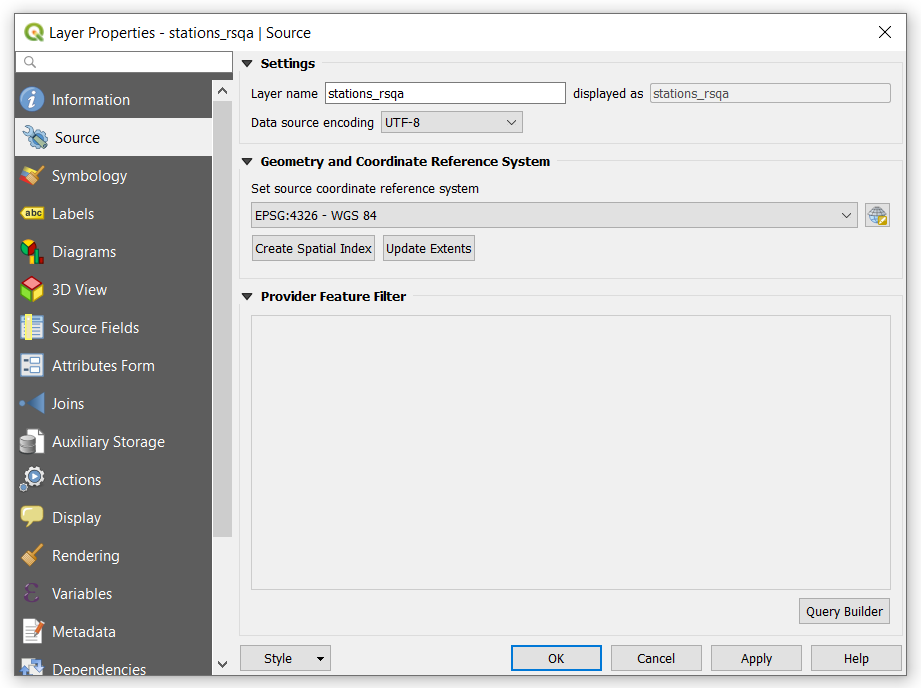
\includegraphics[width=12.79in]{figures/Change_Encoding_2} 

}

\caption{Changing encoding}\label{fig:unnamed-chunk-13}
\end{figure}

Now, import the \texttt{pollutants\_average\_12\_31\_2019\_13H.csv}
file. One kick method is to drag and drop the file from the file into
QGIS. This works fine for this file; however, you also can use
\textbf{Add Delimited Text Layer} to have more control on the
importation.

The \texttt{pollutants\_average\_12\_31\_2019\_13H.csv} file reports the
average concentration of criteria pollutants from December 23, 2013, at
12h. The units of concentration are indicated in the following table.

\begin{longtable}[]{@{}ll@{}}
\toprule
Pollutant & Unit\tabularnewline
\midrule
\endhead
CO & ppm\tabularnewline
H2S & ppb\tabularnewline
NO & ppb\tabularnewline
NO2 & ppb\tabularnewline
SO2 & \(\mu g/m^3\)\tabularnewline
PM10 & \(\mu g/m^3\)\tabularnewline
PM2.5 & \(\mu g/m^3\)\tabularnewline
O3 & ppb\tabularnewline
\bottomrule
\end{longtable}

In order to join the \texttt{pollutants\_average\_12\_31\_2019\_13H}
attribute table to the \texttt{stations\_rsqa} layer, follow these
steps:

\begin{enumerate}
\def\labelenumi{\arabic{enumi}.}
\tightlist
\item
  Right-click on the name of \texttt{stations\_rsqa} layer, select
  \textbf{Properties}, then \textbf{Joins} from the dialog window.
\end{enumerate}

\begin{figure}

{\centering 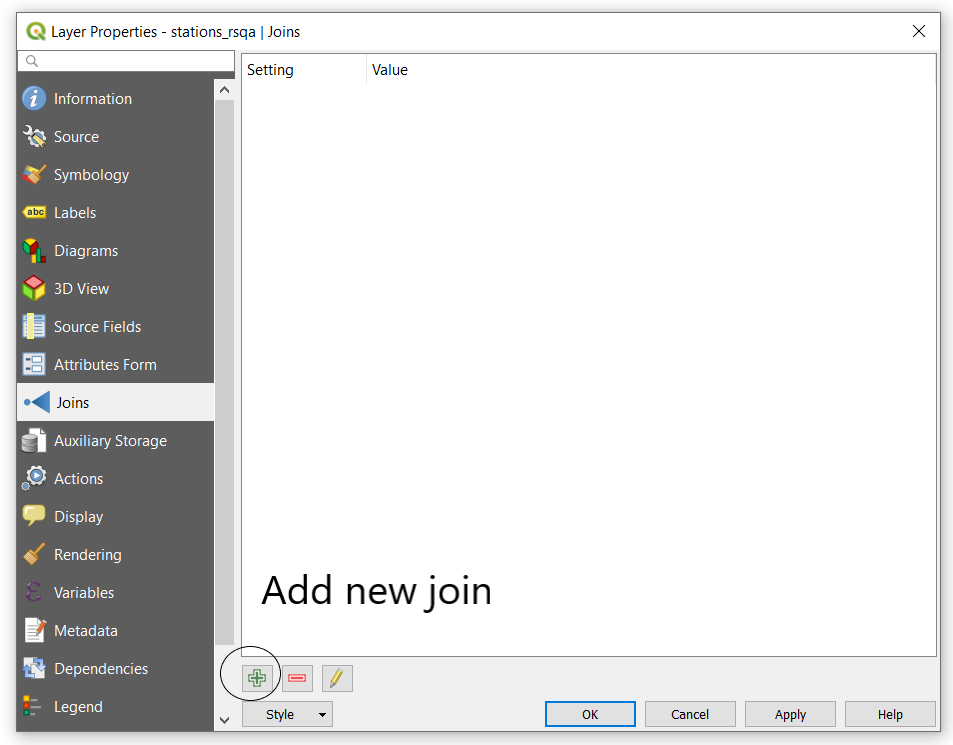
\includegraphics[width=13.24in]{figures/Joins_Dialog_Box} 

}

\caption{Layer properties window}\label{fig:unnamed-chunk-14}
\end{figure}

\begin{enumerate}
\def\labelenumi{\arabic{enumi}.}
\setcounter{enumi}{1}
\tightlist
\item
  Click on the green \textbf{+} sign. The following window will pop up:
\end{enumerate}

\begin{figure}

{\centering 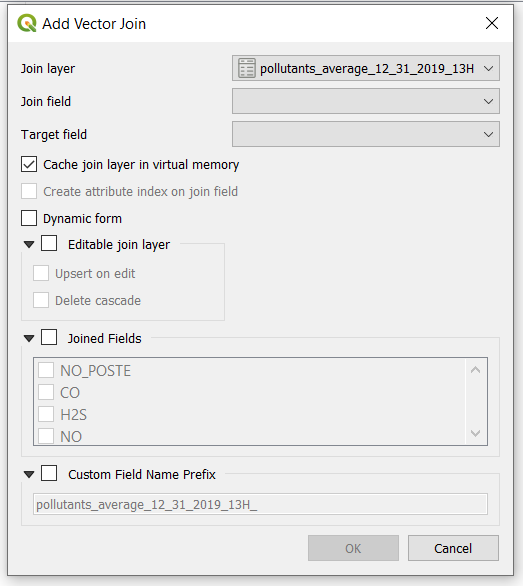
\includegraphics[width=7.26in]{figures/Joins_Dialog_Box_2} 

}

\caption{Joining a layer table}\label{fig:unnamed-chunk-15}
\end{figure}

In this case, since we have imported only one attribute table, QGIS has
already selected the Join layer.

\begin{enumerate}
\def\labelenumi{\arabic{enumi}.}
\setcounter{enumi}{2}
\item
  Specify the \textbf{Join field} and the \textbf{Target field}, which
  correspond to the keys that relate the shapefile layer and the data
  layer. In this example, \textbf{NO\_POSTE} is the identifier of the
  stations in the data layer and \textbf{Numéro st} is the identifier of
  the stations in the shapefile layer. Furthermore, it is possible to
  select the fields that will be joined, and the prefix that will be
  used. Since there are no repeated columns, we just deleted the default
  prefix, which corresponds to the name of the layer.
\item
  Click on \textbf{OK}, then on \textbf{Apply} to finish the joining.
\end{enumerate}

\begin{quote}
To verify if the join has worked, you can open the attribute table of
the shapefile. To make this change permanent, you need to export the
layer. After the join, the layer was exported as
\texttt{stations\_rsqa\_12\_31\_2013.shp}.
\end{quote}

\section{Cleaning up the attribute
table}\label{cleaning-up-the-attribute-table}

Sometimes, data imported into QGIS is not in the correct format, the
name of columns is not self-explanatory, or we simply want to discard
the columns that will not be used during the task in hand.

The \textbf{Refactor fields} algorithm simplifies removing, renaming and
converting the format of dbf tables in QGIS. This algorithm ca be
accessed through the \textbf{Processing Toolbox}. The use of
\textbf{Refactor fields} is illustrated with the
\texttt{stations\_rsqa\_12\_31\_2013.shp} file that was generated in the
previous section.

\begin{enumerate}
\def\labelenumi{\arabic{enumi}.}
\tightlist
\item
  Import \texttt{stations\_rsqa\_12\_31\_2013.shp} file
\item
  Launch the \textbf{Refactor field}. It will detect the available layer
  in the current project. In this window we can identify the name of
  columns, the type of information they store, their length and
  precision. The columns corresponding to concentrations, such as CO,
  H2S, and NO, are currently stored as text (data type is string). This
  is not convenient, since we cannot do arithmetic with text.
  Furthermore, we may want to change the name of \textbf{Numéro st}
  field for \textbf{Station}.
\end{enumerate}

\begin{figure}

{\centering 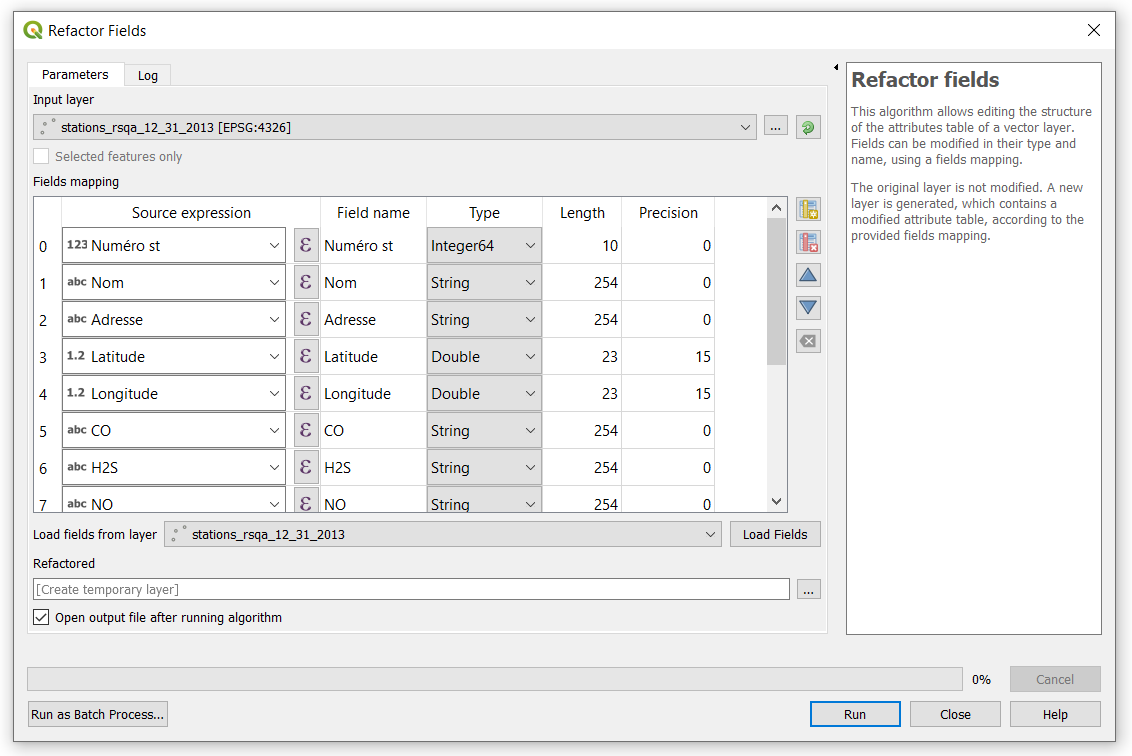
\includegraphics[width=15.72in]{figures/Refactor_Dialog} 

}

\caption{Refactor field window}\label{fig:unnamed-chunk-16}
\end{figure}

\begin{enumerate}
\def\labelenumi{\arabic{enumi}.}
\setcounter{enumi}{2}
\tightlist
\item
  We change the name of the first three columns according to the
  following figure, and the type of columns corresponding to
  concentrations was set as \textbf{Double} (real number) with a length
  of 23 and a precision of 3. Click on \textbf{Run} to generate a new
  layer.
\end{enumerate}

\begin{figure}

{\centering 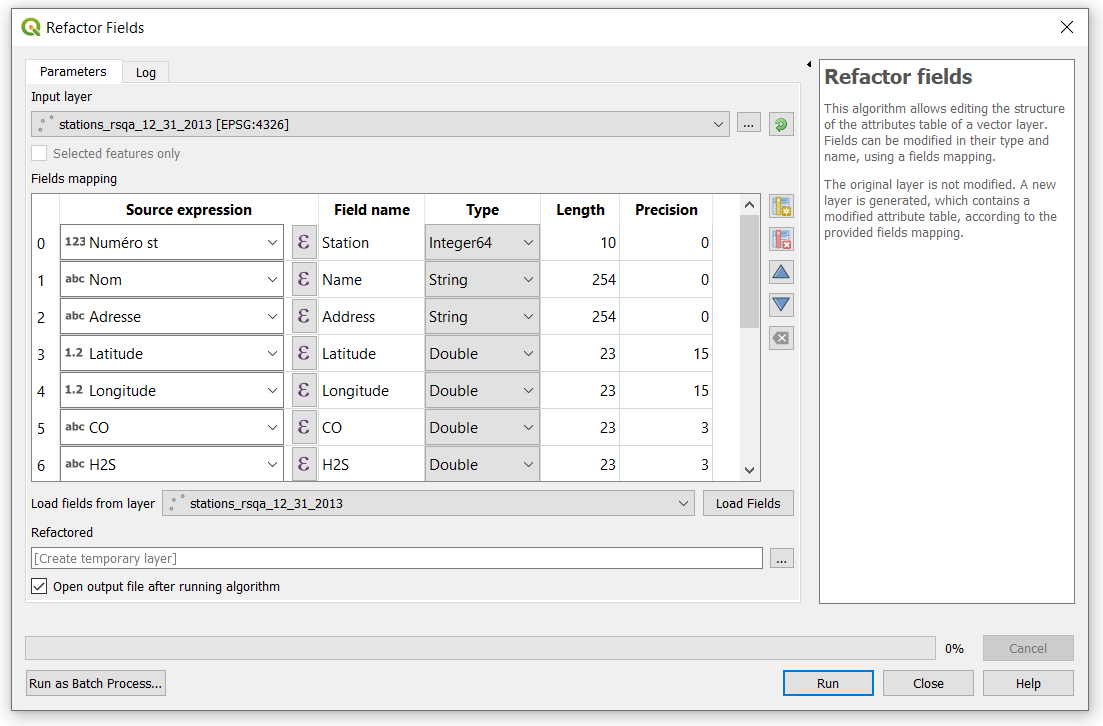
\includegraphics[width=15.32in]{figures/Refactor_Dialog_Settings} 

}

\caption{Using the refactor field algorithm}\label{fig:unnamed-chunk-17}
\end{figure}

\begin{enumerate}
\def\labelenumi{\arabic{enumi}.}
\setcounter{enumi}{3}
\tightlist
\item
  The generated layer is named by default Refactored, of course, you can
  change its name at your convenience.
\end{enumerate}

\begin{figure}

{\centering 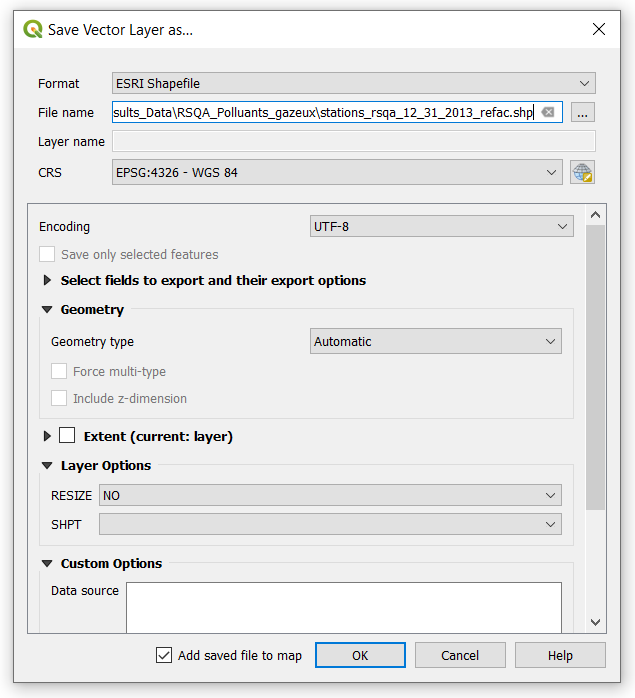
\includegraphics[width=8.82in]{figures/Refactor_Dialog_Settings_2} 

}

\caption{Saving the refactored layer}\label{fig:unnamed-chunk-18}
\end{figure}

\chapter{Data preprocessing steps}\label{data-preprocessing-steps}

\section{Clipping vectors}\label{clipping-vectors}

In some cases, it is necessary than a layer covers only an area of
interest. For this purpose, we can use a layer setting the extent we
want to keep for a section of a layer. To accomplish this task, we use
\textbf{Clip} from the \textbf{Geoprocessing Tool}.

To illustrate the operation of clipping vectors, we will use
\texttt{terre\_shp} and \texttt{LIMADMIN.shp} files.

\begin{enumerate}
\def\labelenumi{\arabic{enumi}.}
\tightlist
\item
  Load both layers into QGIS. \texttt{LIMADMIN.shp} corresponds to the
  administrative limits of Montreal's boroughs (last update in 2013);
  however, the polygons extent beyond the terrestrial limits; whereas
  the \texttt{terre\_shp} file corresponds to the terrestrial limits of
  Montreal Island.
\end{enumerate}

\begin{figure}

{\centering 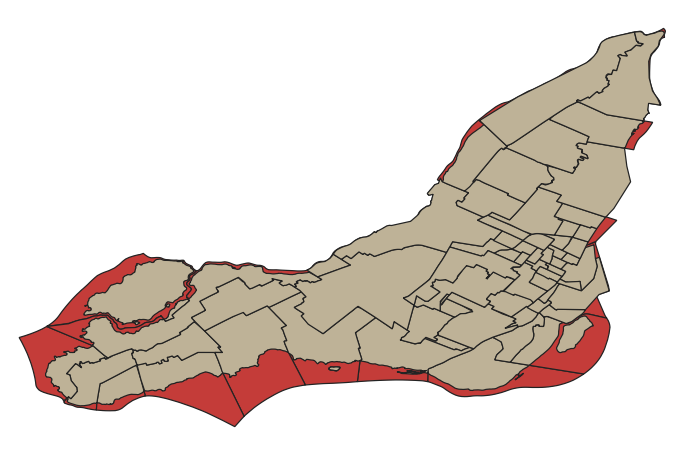
\includegraphics[width=10.25in]{figures/Clipping_Vectors} 

}

\caption{Montreal’s boroughs}\label{fig:unnamed-chunk-19}
\end{figure}

\begin{enumerate}
\def\labelenumi{\arabic{enumi}.}
\setcounter{enumi}{1}
\tightlist
\item
  Navigate to \textbf{Layer}, then to \textbf{Geoprocessing Tool}, and
  select \textbf{Clip}. The following window will pop up.
  \texttt{LIMADMIN.shp} layer corresponds to the Input layer, since it
  is the layer we want to cut, whereas the \texttt{quartier\_limite.shp}
  is the Overlay layer, the layer we will use to set the limits we want
  to keep.
\end{enumerate}

\begin{figure}

{\centering 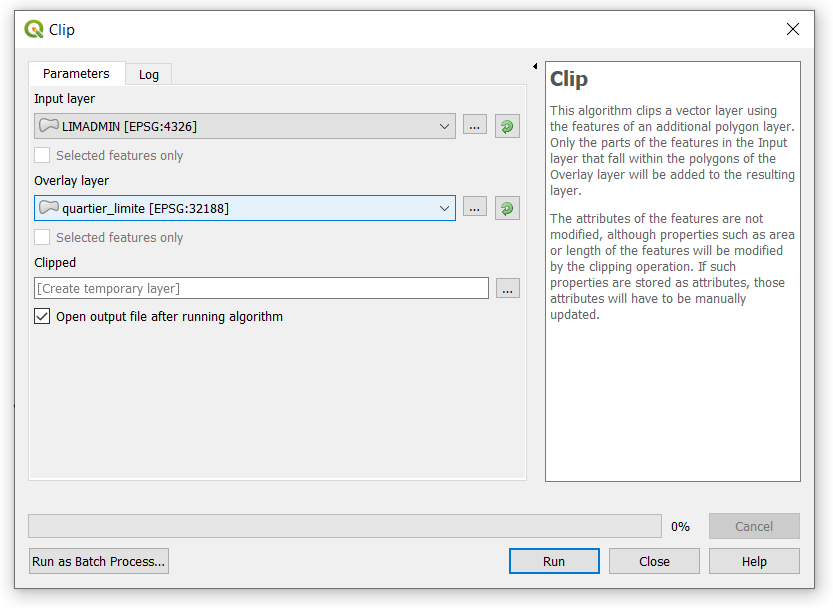
\includegraphics[width=10.6in]{figures/Clipping_Vectors_Dialog} 

}

\caption{Using the clip algorithm}\label{fig:unnamed-chunk-20}
\end{figure}

\begin{enumerate}
\def\labelenumi{\arabic{enumi}.}
\setcounter{enumi}{3}
\tightlist
\item
  Click on Run to generate a new layer. Save the clipped layer as
  \texttt{limadmin\_clipped.shp}.
\end{enumerate}

\section{Intersecting vectors}\label{IntersectionVectors}

The \textbf{Intersection} algorithm extracts the properties from the
input layer that overlap features in the overlay layer.

To illustrate this recipe, consider the \texttt{terre.shp} and
\texttt{LIMADMIN.shp} files. In this case, we will create a layer
resulting from the intersection between \texttt{terre.shp} and
\texttt{LIMADMIN.shp}. Therefore, the \texttt{terre.shp} layer
corresponds to the \textbf{Input Layer}, whereas \texttt{LIMADMIN.shp}
to the \textbf{Overlay Layer}. We can add an overlay index to identify
the features that were intersected from the overlay layer in
Intersection layer generated

\begin{figure}

{\centering 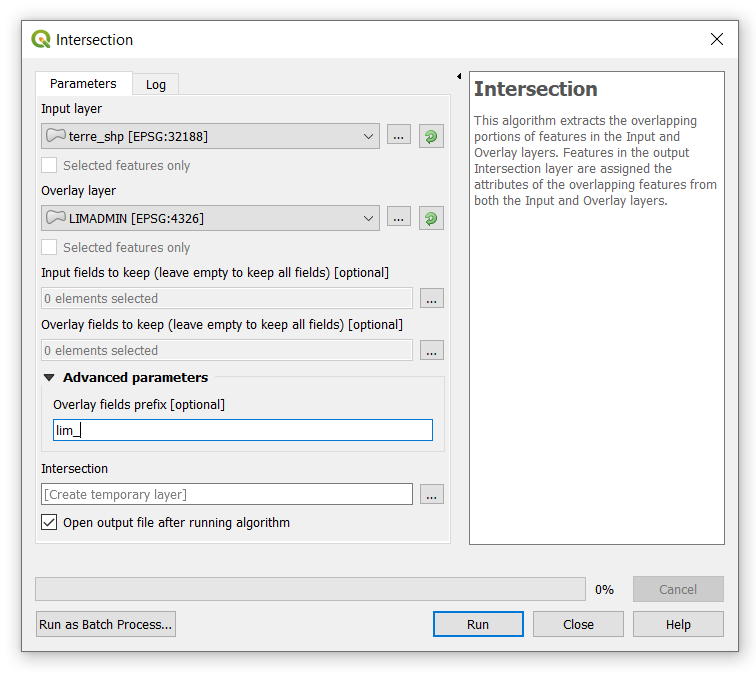
\includegraphics[width=10.5in]{figures/Intersecting_Vectors_Dialog} 

}

\caption{Intersection of vectors}\label{fig:unnamed-chunk-21}
\end{figure}

\section{Check validity and fix
geometries}\label{check-validity-and-fix-geometries}

In some cases, when clipping and intersecting vectors, errors may arise
because of invalid geometries. Fortunately, QGIS allows us to check the
validity of layers, and even more importantly to fix them. The following
algorithms can be accessed through the \textbf{Processing Toolbox}:

\begin{itemize}
\tightlist
\item
  \textbf{Check validity}: The algorithm performs a validity check on
  the geometries of a vector layer. The geometries are classified in
  three groups (valid, invalid and error).
\item
  \textbf{Fix geometries}: The algorithm attempts to create a valid
  representation of an invalid geometry without losing any of the input
  vertices.
\end{itemize}

\begin{figure}

{\centering 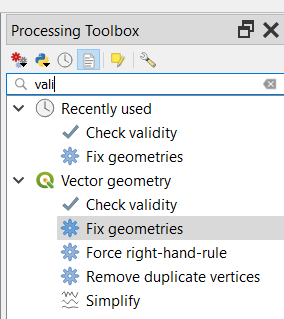
\includegraphics[width=3.94in]{figures/Validity_Fix_Geometry} 

}

\caption{Check validity and fix geometries}\label{fig:unnamed-chunk-22}
\end{figure}

\chapter{Data exploration}\label{data-exploration}

\section{Listing unique values in a
column}\label{listing-unique-values-in-a-column}

The \textbf{List Unique values} algorithm, from the \textbf{Processing
Toolbox}, generates a table and a HTLM report of the unique values of a
given layer's field.

To illustrate the use of the \textbf{List Unique values} algorithm, we
will import the \texttt{grandparcs.kml} file. The field
\textbf{Generique2} stores the type of parks located in Montreal, and we
would like to know the unique values without having to open the
attribute table.

\begin{enumerate}
\def\labelenumi{\arabic{enumi}.}
\item
  Launch the \textbf{List Unique values} algorithm from the
  \textbf{Processing Toolbox}. It will identify the available layer in
  the current project.
\item
  Click on \textbf{\ldots{}} from the \textbf{Target Field(s)} and
  select \textbf{Generique2}. Click on Run to generate a temporary layer
  and a HTLM report.
\end{enumerate}

\begin{figure}

{\centering 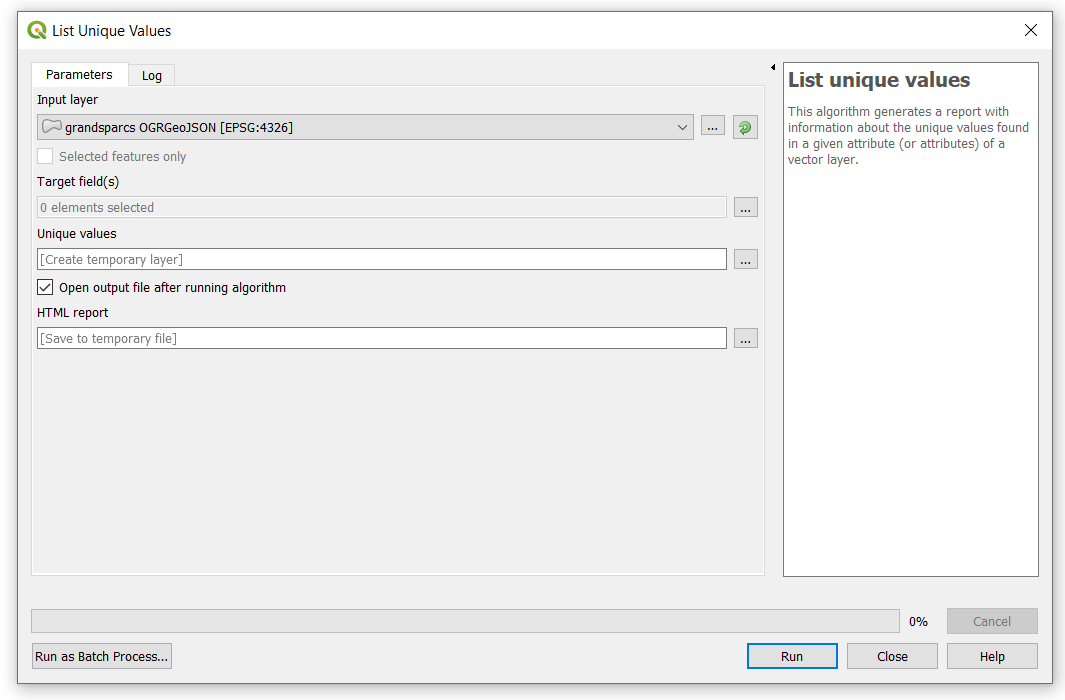
\includegraphics[width=14.79in]{figures/List_Unique_Values} 

}

\caption{List unique values window}\label{fig:unnamed-chunk-23}
\end{figure}

\section{Loading BaseMaps}\label{basemaps}

When we import layers into QGIS, sometimes it is difficult to identify
what the points, lines or polygons of a layer correspond to. In these
situations, it is very helpful to add a base map to give some spatial
context.

One plugging that comes in hand to add spatial context is
\textbf{QuickMapServices}. If it is not already available in your QGIS
Desktop, navigate to \textbf{Plugins}, then to \textbf{Manage and
Install Plugins}. In the window that has been displayed search
\textbf{QuickMapServices} and click on \textbf{Install Plugin}.

\begin{figure}

{\centering 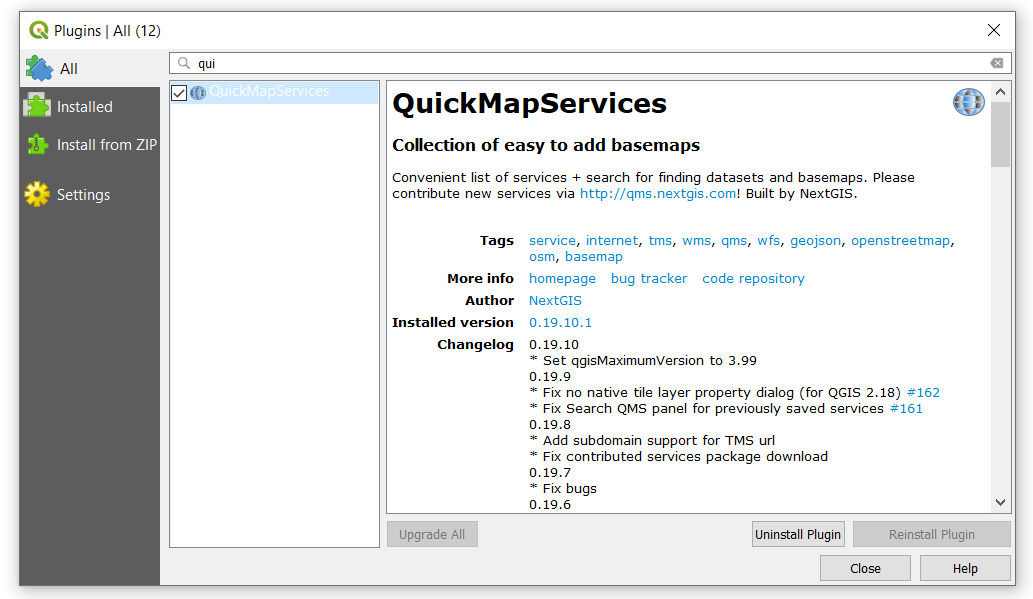
\includegraphics[width=14.35in]{figures/QuickMapServices} 

}

\caption{Manage and install plugins in QGIS}\label{fig:unnamed-chunk-24}
\end{figure}

To illustrate the use of \textbf{QuickMapServices}, load the
\texttt{stations\_rsqa\_12\_31\_2013.shp}. Navigate to \textbf{Web} from
the menu bar, select \textbf{QuickMapServices}, go to \textbf{OSM}, and
select \textbf{OSM\_Standard}. You will see the following set of air
quality monitoring stations located in Montreal.

\begin{figure}

{\centering 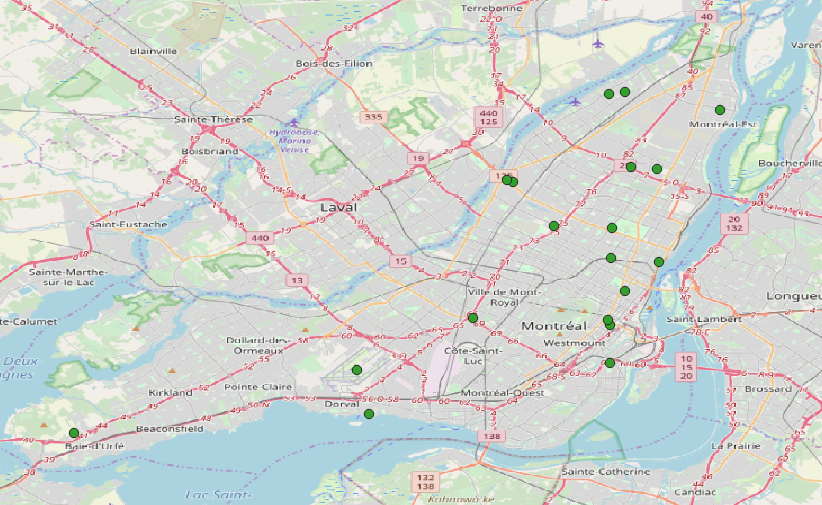
\includegraphics[width=11.42in]{figures/BaseMaps_Example} 

}

\caption{Montreal's Air Quality Monitoring Network}\label{fig:unnamed-chunk-25}
\end{figure}

\chapter{Exercises}\label{exercises}

\section{Exercise 1: Determine the area fraction of urban heat islands
by boroughs of
Montreal}\label{exercise-1-determine-the-area-fraction-of-urban-heat-islands-by-boroughs-of-montreal}

The aim of this exercise is to generate a
\href{https://en.wikipedia.org/wiki/Choropleth_map}{choropleth map}
showing the area fraction of urban heat islands by boroughs of Montreal.

\begin{figure}

{\centering 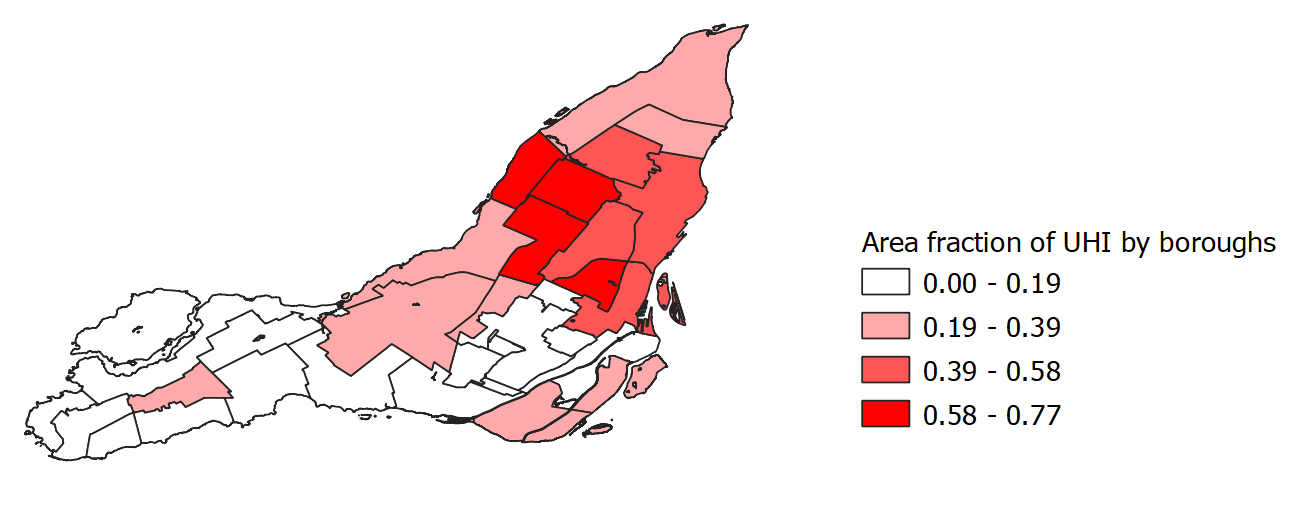
\includegraphics[width=18.1in]{figures/Choropleth_UHI} 

}

\caption{Area fraction of UHI by boroughs}\label{fig:unnamed-chunk-26}
\end{figure}

\begin{enumerate}
\def\labelenumi{\arabic{enumi}.}
\tightlist
\item
  Import \texttt{ilotschaleur.json} and \texttt{limadmim\_clipped.shp}.
\end{enumerate}

\begin{figure}

{\centering 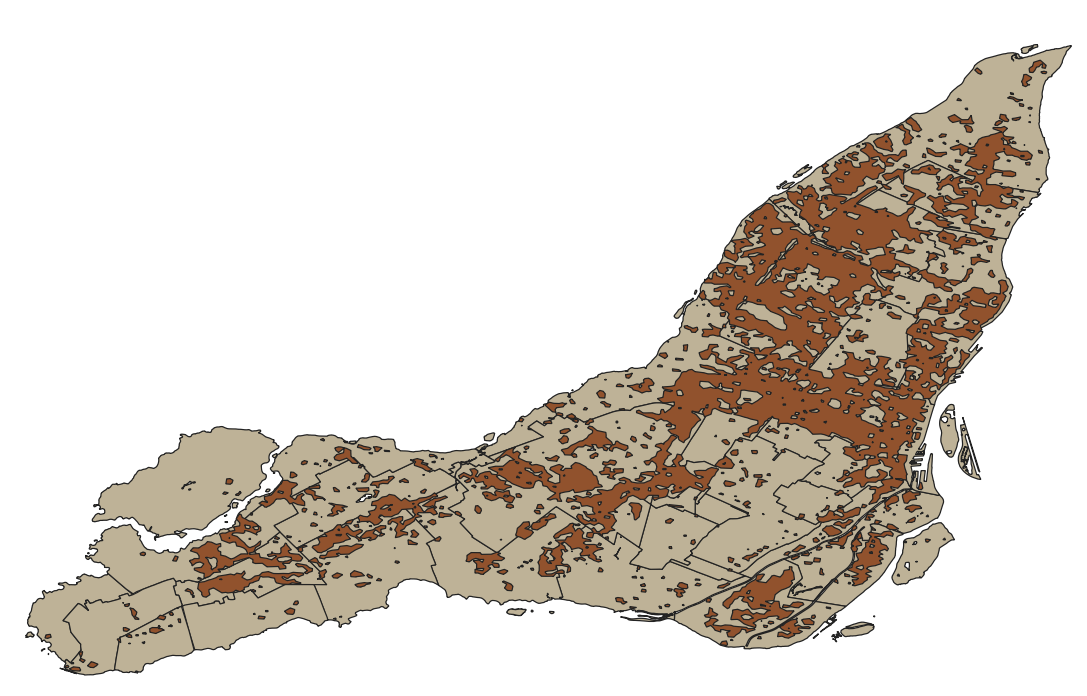
\includegraphics[width=15.1in]{figures/UHA_Montreal} 

}

\caption{UHI and boroughs of Montreal}\label{fig:unnamed-chunk-27}
\end{figure}

\begin{enumerate}
\def\labelenumi{\arabic{enumi}.}
\setcounter{enumi}{1}
\item
  Export \texttt{ilotschaleur.json} as a shapefile and save it as
  \texttt{ilotschaleur.shp} (Section \ref{saveLayer}).
\item
  Intersect the recently created layer \texttt{ilotschaleur.shp} with
  \texttt{limadmim\_clipped.shp}. Navigate to \textbf{Vector}, select
  \textbf{Geoprocessing Tools}, and the \textbf{Intersection} (Section
  \ref{IntersectionVectors}). Set the following parameters:
\end{enumerate}

\begin{itemize}
\tightlist
\item
  \textbf{Input layer}: \texttt{ilotschaleur.shp}
\item
  \textbf{Overlay layer}: \texttt{limadmim\_clipped.shp}
\end{itemize}

The aim is to generate a new layer in which the urban heat islands are
divided according to Montreal's boroughs.

\begin{figure}

{\centering 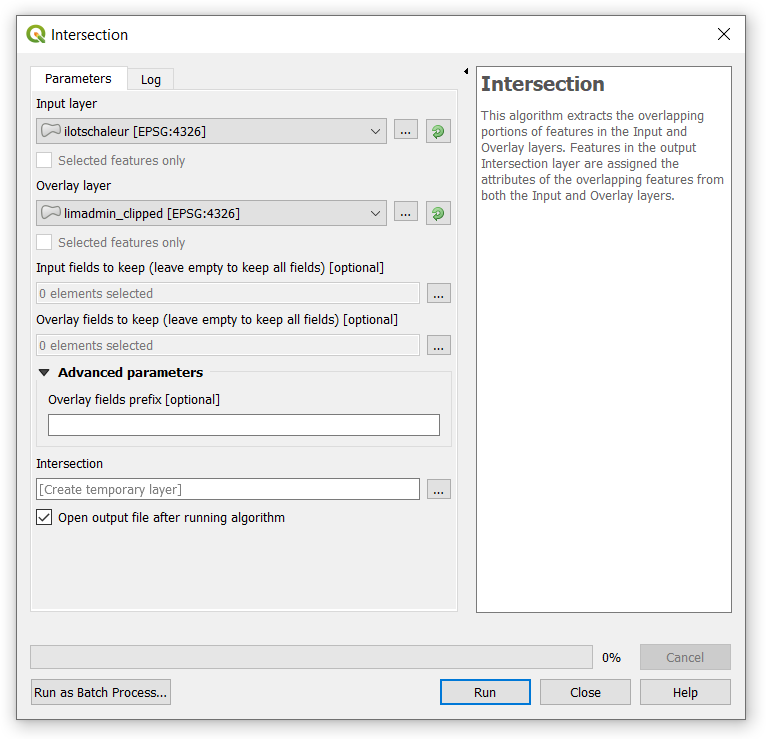
\includegraphics[width=10.64in]{figures/Intersection_UHA} 

}

\caption{Intersection of layers}\label{fig:unnamed-chunk-28}
\end{figure}

Click Run to execute the algorithm. However, it will stop since there
are some invalid geometries in the input layer.

\begin{figure}

{\centering 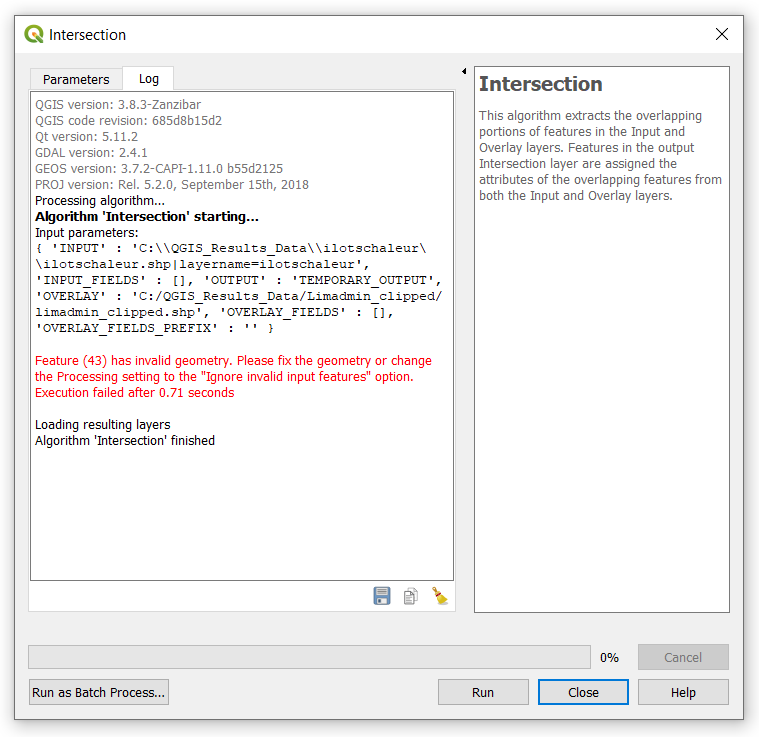
\includegraphics[width=10.54in]{figures/Intersection_UHA_Error} 

}

\caption{Error: Intersection of layers}\label{fig:unnamed-chunk-29}
\end{figure}

\begin{enumerate}
\def\labelenumi{\arabic{enumi}.}
\setcounter{enumi}{3}
\tightlist
\item
  We will use the \textbf{Fix Geometries} algorithm from the
  \textbf{Processing Toolbox} to fix the geometries. Run the algorithm
  according to the following settings.
\end{enumerate}

\begin{figure}

{\centering 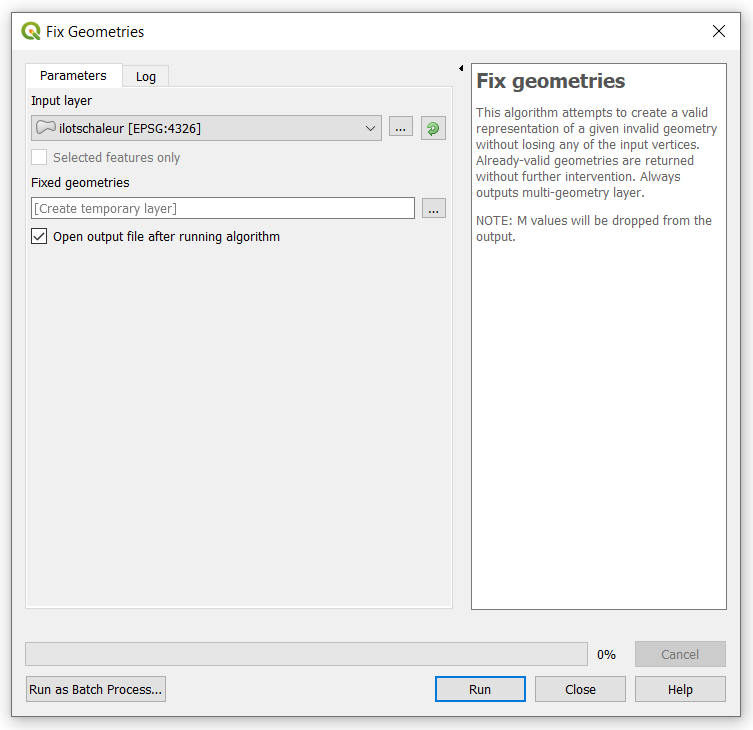
\includegraphics[width=10.46in]{figures/Fix_Geometry_UHA} 

}

\caption{Fix geometries algorithm}\label{fig:unnamed-chunk-30}
\end{figure}

A temporary layer will be generated after running the algorithm. Right
click on layer \texttt{Fixed\ geometries} and rename it
\texttt{ilotschaleur\_fixed}.

\begin{enumerate}
\def\labelenumi{\arabic{enumi}.}
\setcounter{enumi}{4}
\tightlist
\item
  Run again the \textbf{Intersection} algorithm, but this time use the
  fixed layer of urban heat islands. Set the following parameters:
\end{enumerate}

\begin{itemize}
\tightlist
\item
  \textbf{Input layer}: \texttt{ilotschaleur\_fixed.shp}
\item
  \textbf{Overlay layer}: \texttt{limadmim\_clipped.shp}
\end{itemize}

\begin{figure}

{\centering 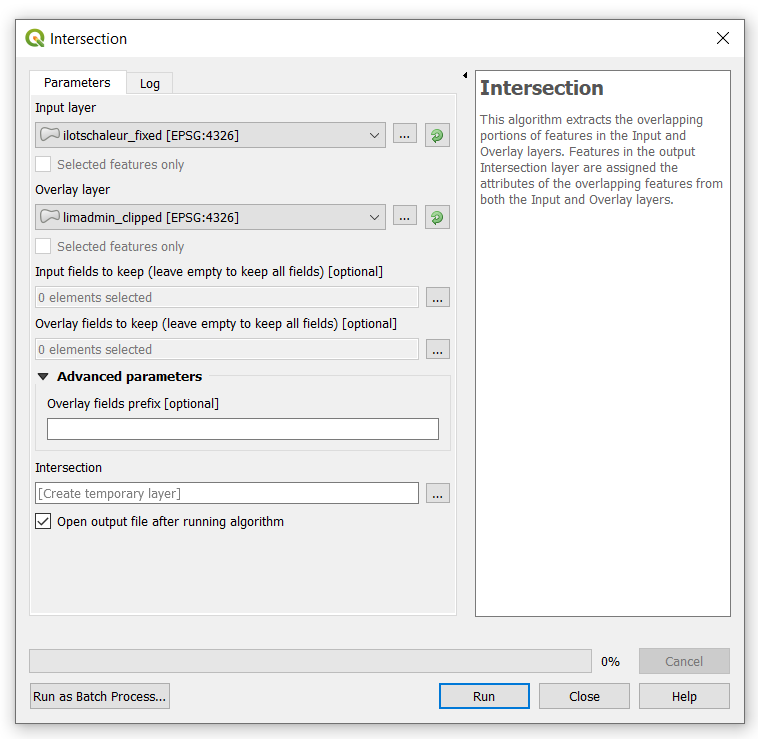
\includegraphics[width=10.53in]{figures/Intersection_UHA_Fixed} 

}

\caption{Intersection of layers}\label{fig:unnamed-chunk-31}
\end{figure}

A temporary layer \texttt{Intersection} will be generated after running
the algorithm. To verify that the algorithm has properly worked, open
the attribute table and you will notice that the \texttt{Intersection}
layer has 584 attributes, whereas the \texttt{ilotschaleur\_fixed} has
498.

\begin{enumerate}
\def\labelenumi{\arabic{enumi}.}
\setcounter{enumi}{5}
\tightlist
\item
  Dissolve the \texttt{Intersection} layer by NOM. The aim is to combine
  the polygons corresponding to the same borough, which is given by the
  NOM field. In the \textbf{Dissolve field(s)}, click on the \ldots{}
  and select NOM.
\end{enumerate}

\begin{figure}

{\centering 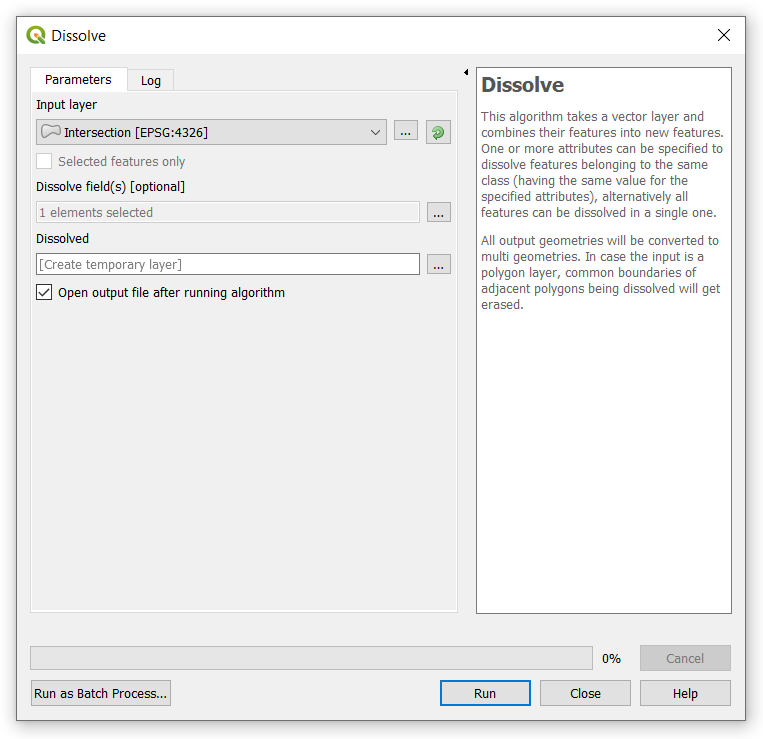
\includegraphics[width=10.6in]{figures/Dissolve_UHA} 

}

\caption{Dissolve Intersection layer by NOM}\label{fig:unnamed-chunk-32}
\end{figure}

After running the \textbf{Dissolve} algorithm, a temporary layer
\texttt{Dissolved} will be generated. Open the attribute table of this
layer and verify that it has 33 attributes; whereas the
\texttt{Intersection} layer has 584. The task of combining the polygons
has been accomplished.

\begin{enumerate}
\def\labelenumi{\arabic{enumi}.}
\setcounter{enumi}{6}
\tightlist
\item
  Calculate the area of the urban heat islands by boroughs.
\end{enumerate}

First of all, we will delete the fields of the \texttt{Dissolved} layer
that will not be used. Open the attribute table, then click on the
pencil shown in the left corner (\textbf{Toggle editing mode}) to allow
editing the attribute table. Click on \textbf{Delete} field and select
the fields shown in the following figure:

\begin{figure}

{\centering 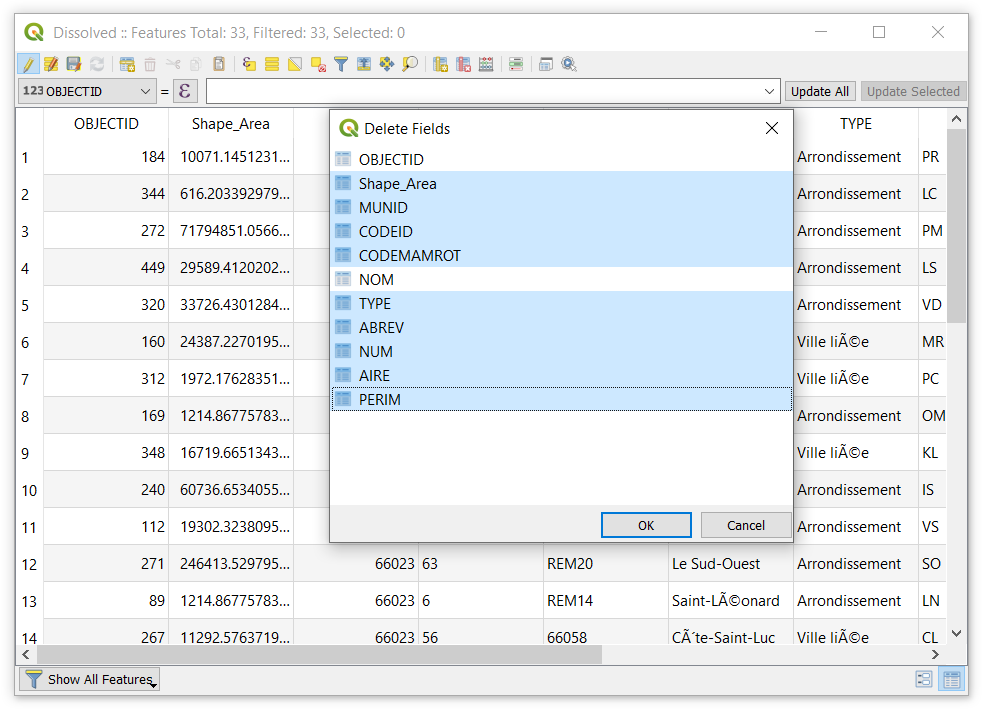
\includegraphics[width=13.75in]{figures/Delete_Fields} 

}

\caption{Delete some fields of Dissolved layer}\label{fig:unnamed-chunk-33}
\end{figure}

We will now calculate the area of the urban heat islands by borough.
Click on \textbf{New field}. In the window that will display, select
\textbf{Create a new field}, indicate \emph{AREA} in the \textbf{Output
field name}, set \emph{Decimal number (real)} as the \textbf{Output
field type}. Double click on \emph{\$area} from the center panel.

\begin{figure}

{\centering 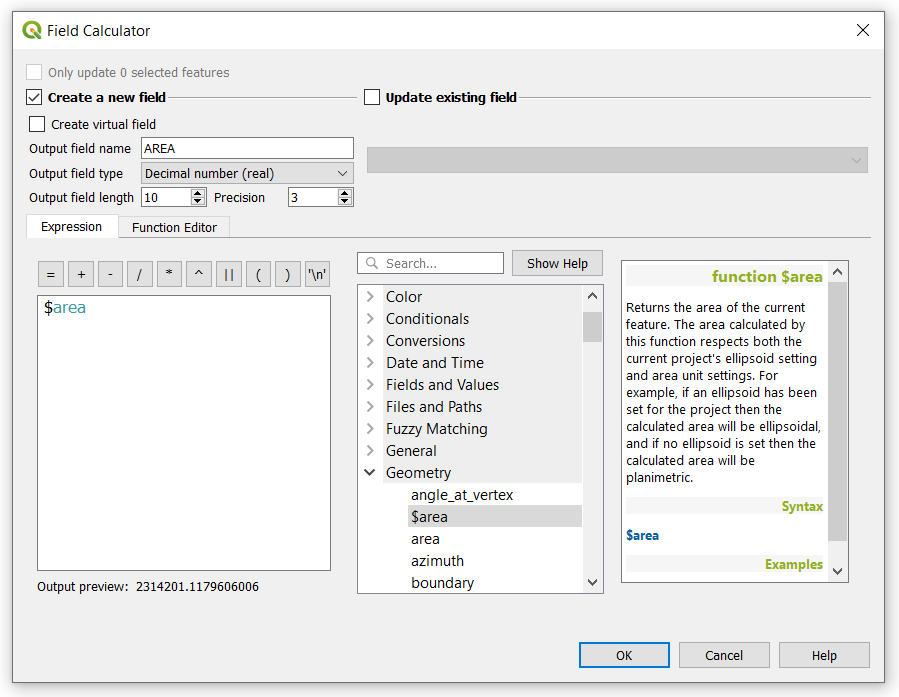
\includegraphics[width=12.49in]{figures/Calculate_Area} 

}

\caption{Calculate the area of UHI}\label{fig:unnamed-chunk-34}
\end{figure}

\begin{enumerate}
\def\labelenumi{\arabic{enumi}.}
\setcounter{enumi}{7}
\tightlist
\item
  Join the AREA of the urban heat islands (\texttt{Dissolved} layer) to
  the respective borough in the \texttt{limadmim\_clipped.shp} layer.
  The prefix \textbf{UHA\_ was} set to distinguish the fields from the
  joined layer.
\end{enumerate}

\begin{figure}

{\centering 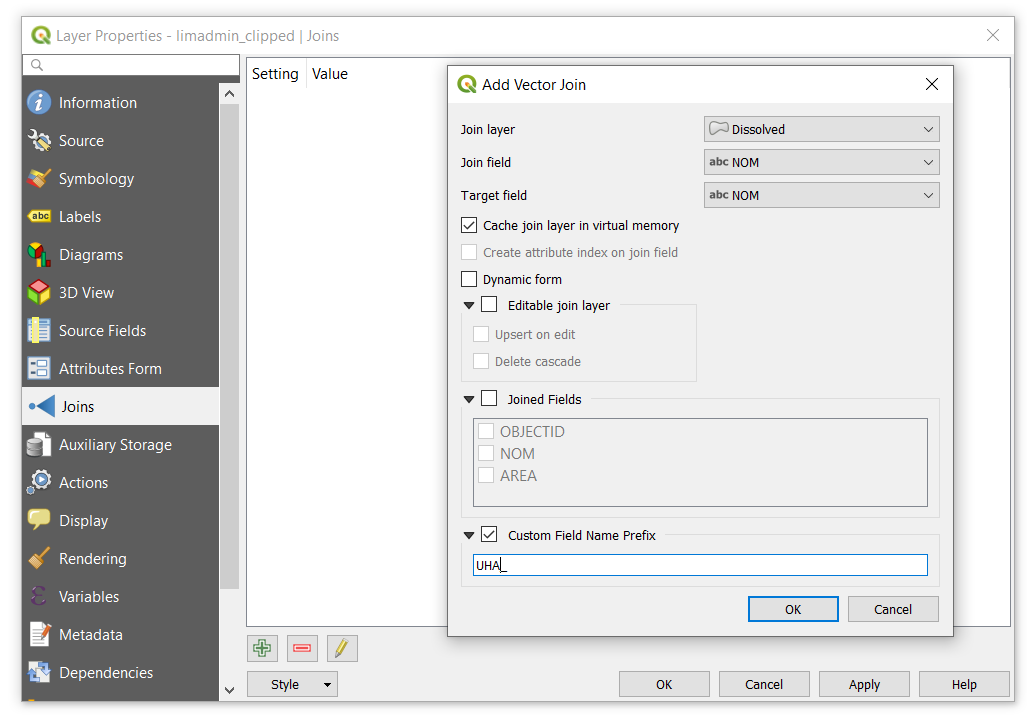
\includegraphics[width=14.26in]{figures/Join_UHA} 

}

\caption{Join layers}\label{fig:unnamed-chunk-35}
\end{figure}

\begin{enumerate}
\def\labelenumi{\arabic{enumi}.}
\setcounter{enumi}{8}
\tightlist
\item
  Calculate the fraction area of urban heat islands (UHI) by boroughs.
\end{enumerate}

First, calculate the AREA of each borough from the
\texttt{limadmim\_clipped.shp} layer. Click on \textbf{New field}. In
the window that will display, select \textbf{Create a new field},
indicate AREA in the Output field name, set Decimal number (real) as the
Output field type. Double click on \$area from the center panel.

\begin{figure}

{\centering 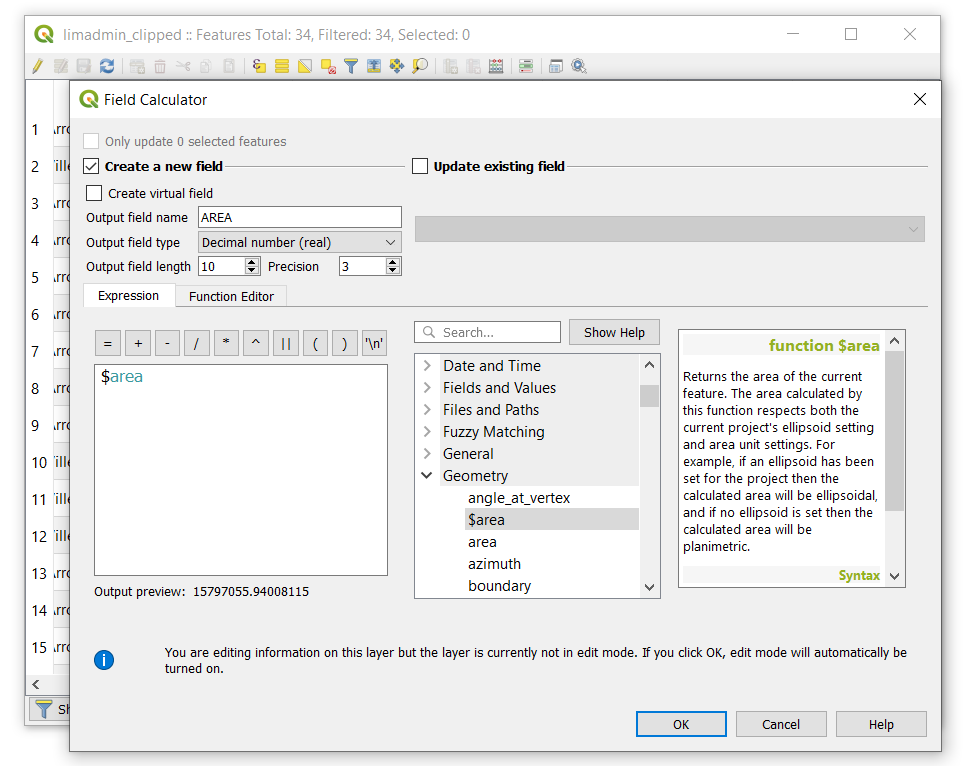
\includegraphics[width=13.42in]{figures/Calculate_Area_Montreal} 

}

\caption{Calculate the area of Montreal's boroughs}\label{fig:unnamed-chunk-36}
\end{figure}

Finally, calculate the area fraction of UHI. In the center panel, go to
\textbf{Fields and Values}, double click to select the involved fields
in the computation of the new one. In this case, the area fraction is
given by the expression: FRAC\_UHA = UHA\_AREA/AREA

\begin{quote}
Note: UHI was misspelled. So UHA stand for UHI.
\end{quote}

\begin{figure}

{\centering 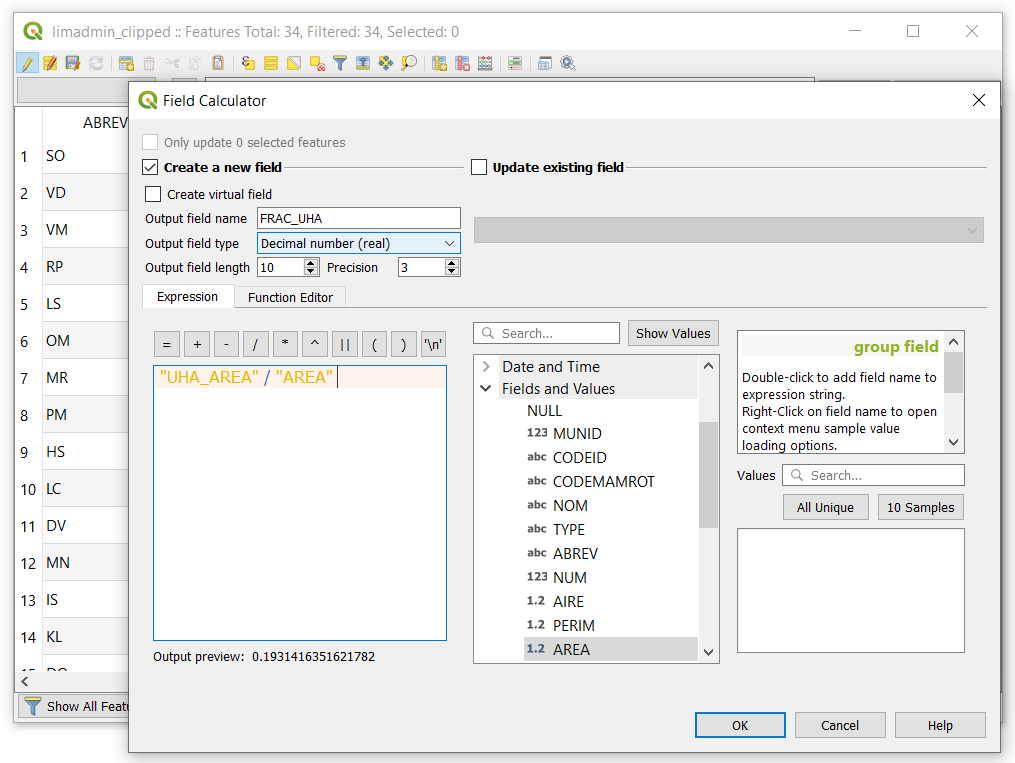
\includegraphics[width=14.1in]{figures/Calculate_Area_Fraction} 

}

\caption{Calculate the area fraction of UHI}\label{fig:unnamed-chunk-37}
\end{figure}

\begin{enumerate}
\def\labelenumi{\arabic{enumi}.}
\setcounter{enumi}{9}
\tightlist
\item
  Style the \texttt{limadmim\_clipped.shp} layer so that it shows the
  area fraction of UHI in four classes of equal interval.
\end{enumerate}

Right click on \texttt{limadmim\_clipped.shp}, select
\textbf{Properties}, then \textbf{Symbology}, and set the parameters
according to the following figure.

\begin{figure}

{\centering 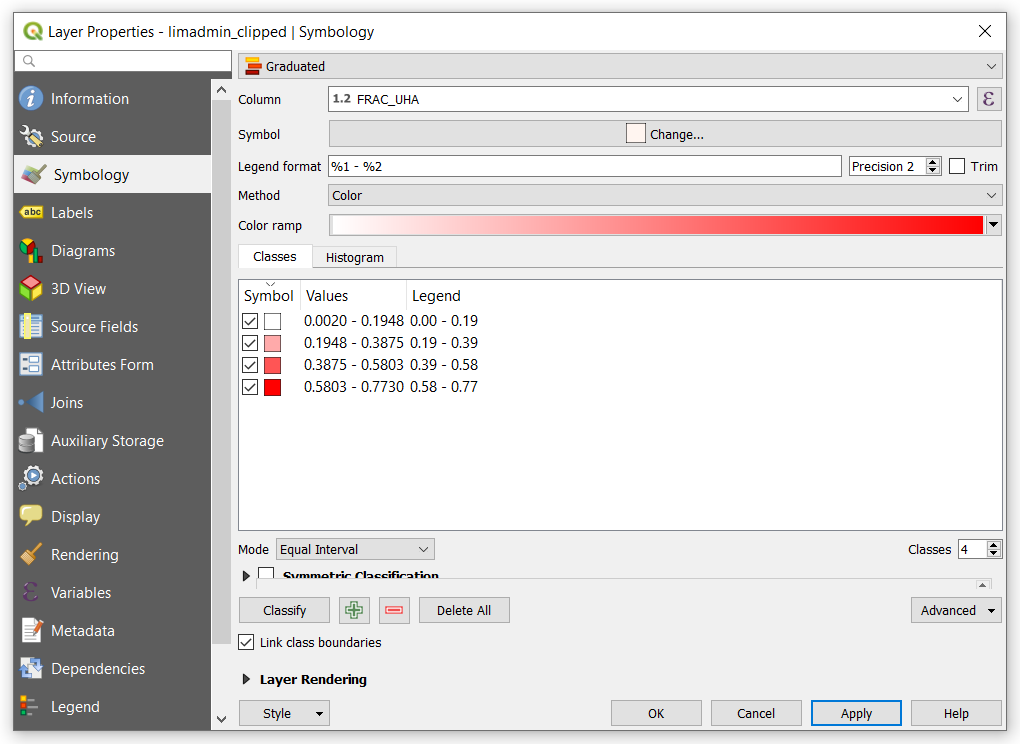
\includegraphics[width=14.17in]{figures/Area_Fraction_UHA} 

}

\caption{Changing the symbology of a layer}\label{fig:unnamed-chunk-38}
\end{figure}

\chapter{References}\label{references}

\begin{longtable}[]{@{}lll@{}}
\toprule
\begin{minipage}[b]{0.08\columnwidth}\raggedright\strut
Data\strut
\end{minipage} & \begin{minipage}[b]{0.16\columnwidth}\raggedright\strut
File name\strut
\end{minipage} & \begin{minipage}[b]{0.10\columnwidth}\raggedright\strut
Source\strut
\end{minipage}\tabularnewline
\midrule
\endhead
\begin{minipage}[t]{0.08\columnwidth}\raggedright\strut
RSQA - liste des stations\strut
\end{minipage} & \begin{minipage}[t]{0.16\columnwidth}\raggedright\strut
coordonnees-stations-rsqa.csv\strut
\end{minipage} & \begin{minipage}[t]{0.10\columnwidth}\raggedright\strut
\href{http://donnees.ville.montreal.qc.ca/dataset/rsqa-liste-des-stations/resource/29db5545-89a4-4e4a-9e95-05aa6dc2fd80}{Portail
données ouvertes Montréal}\strut
\end{minipage}\tabularnewline
\begin{minipage}[t]{0.08\columnwidth}\raggedright\strut
RSQA - polluants gazeux 2013-07-01 à 2013-12-31\strut
\end{minipage} & \begin{minipage}[t]{0.16\columnwidth}\raggedright\strut
pollutants\_average\_12\_31\_2019\_13H.csv\strut
\end{minipage} & \begin{minipage}[t]{0.10\columnwidth}\raggedright\strut
\href{http://donnees.ville.montreal.qc.ca/dataset/rsqa-polluants-gazeux/resource/26ddbd0b-47f6-4039-98b2-b32568ed01b1}{Portail
données ouvertes Montréal}\strut
\end{minipage}\tabularnewline
\begin{minipage}[t]{0.08\columnwidth}\raggedright\strut
Grands parcs\strut
\end{minipage} & \begin{minipage}[t]{0.16\columnwidth}\raggedright\strut
grandparcs.kml\strut
\end{minipage} & \begin{minipage}[t]{0.10\columnwidth}\raggedright\strut
\href{http://donnees.ville.montreal.qc.ca/dataset/grands-parcs}{Portail
données ouvertes Montréal}\strut
\end{minipage}\tabularnewline
\begin{minipage}[t]{0.08\columnwidth}\raggedright\strut
Îlots de chaleur\strut
\end{minipage} & \begin{minipage}[t]{0.16\columnwidth}\raggedright\strut
ilotschaleur.json\strut
\end{minipage} & \begin{minipage}[t]{0.10\columnwidth}\raggedright\strut
\href{http://donnees.ville.montreal.qc.ca/dataset/schema-environnement-milieux-naturels/resource/8cd8d34a-cfdd-4acf-a363-d4adaeff18c0}{Portail
données ouvertes Montréal}\strut
\end{minipage}\tabularnewline
\begin{minipage}[t]{0.08\columnwidth}\raggedright\strut
Limite administrative de l'agglomération de Montréal (Arrondissement et
Ville liée)\strut
\end{minipage} & \begin{minipage}[t]{0.16\columnwidth}\raggedright\strut
LIMADMIN.shp\strut
\end{minipage} & \begin{minipage}[t]{0.10\columnwidth}\raggedright\strut
\href{http://donnees.ville.montreal.qc.ca/dataset/polygones-arrondissements}{Portail
données ouvertes Montréal}\strut
\end{minipage}\tabularnewline
\begin{minipage}[t]{0.08\columnwidth}\raggedright\strut
Anciens territoires administratifs de l'île de Montréal\strut
\end{minipage} & \begin{minipage}[t]{0.16\columnwidth}\raggedright\strut
quartier\_limite.shp\strut
\end{minipage} & \begin{minipage}[t]{0.10\columnwidth}\raggedright\strut
\href{http://donnees.ville.montreal.qc.ca/dataset/anciens-territoires}{Portail
données ouvertes Montréal}\strut
\end{minipage}\tabularnewline
\bottomrule
\end{longtable}

\bibliography{book.bib,packages.bib}


\end{document}
